\documentclass[conference]{IEEEtran}
\IEEEoverridecommandlockouts
\IEEEpubid{\makebox[\columnwidth]{978-1-7281-8393-0/21/\$31.00~\copyright2021 IEEE \hfill}
  \hspace{\columnsep}\makebox[\columnwidth]{ }
}

% The preceding line is only needed to identify funding in the first footnote. If that is unneeded, please comment it out.
\usepackage{cite}
\usepackage{amsmath,amssymb,amsfonts}
\usepackage{algorithmic}
\usepackage{graphicx}
\usepackage{textcomp}
\usepackage{xcolor}
\usepackage{subfigure}
\usepackage{multirow}
\usepackage{hyperref}

\begin{document}

\title{Random Selection of Parameters in Asynchronous Pool-Based Evolutionary Algorithms}

\author{\IEEEauthorblockN{Mario Garc\'ia-Valdez, Ren\'e M\'arquez, Leonardo Trujillo}
  \IEEEauthorblockA{Instituto Tecnol\'ogico de Tijuana \\
    mario@tectijuana.edu.mx}
  \and
  \IEEEauthorblockN{J.J. Merelo}
  \IEEEauthorblockA{Computer Architecture and Technology\\
    University of Granada, Spain\\
    jmerelo@ugr.es}
}

\maketitle

\IEEEpubidadjcol

\begin{abstract}
  Synchronous operation is not the most natural, as in biologically
  inspired, mode to run
distributed algorithms. In many grid, cloud or volunteer setups nodes
are heterogeneous, or simply are not available at the exact same time;
this is a challenge for the researcher if their full performance is
going to be actually leveraged. Asynchronous distributed evolutionary
algorithms try to solve this by dropping the homogeneity, as well as
the synchronicity, assumption. These algorithms share the population between distributed
workers which execute the actual evolutionary process by taking
samples of the population, and replacing them in the population pool
by evolved individuals. The performance of these EAs depends in part
on the selection of parameters for the EA running in each worker. In
this paper we study how randomly varying parameters in distributed
evolutionary algorithms affects performance. Experiments were
conducted in the AWS cloud using 2, 6 and 12 virtual machine
configurations, with both homogeneous and heterogeneous random
settings using five test functions for real-valued optimization and
the OneMax binary problem. The results suggest that this method can
produce a performance that is competitive with instances of the
algorithm using workers with parameters specially tuned for the
benchmark.
\end{abstract}


\begin{IEEEkeywords}
  Distributed Evolutionary Algorithms, Volunteer Computing,
  Cloud Computing, pool-based evolutionary algorithms, parameter optimization.
\end{IEEEkeywords}

\section{Introduction}

%Why Parallel
Biological evolution is a process with some interesting properties,
with which we can design computational systems, that are asynchronous,
parallel, and distributed; however, it is not trivial to include some
of these characteristics in standard EAs, and many remain as
sequential and synchronous algorithms \cite{eiben}.  A large body of
work exists about the parallelization EAs, using multi-core,
distributed systems, and GPUs
\cite{cantu2000efficient,hofmann2013performance}.  However, only
recently asynchronous and distributed EAs have started to become a
common practice, intending to exploit computing resources available
everywhere from personal computers, smartphones, and tablets, as well
as data centers \cite{agajaj,FlexGP}.

Access to these resources can be easily achieved through popular Internet 
technologies, such as cloud computing, peer-to-peer (P2P), and web environments. 
Moreover, these technologies are intended for the
development of parallel, distributed and asynchronous systems, such
that an EA developed on top of them could easily reap the benefits of
these features.

%Pool Based
The focus of this work is on Pool-based EAs or PEAs. This is a type of
bioinspired algorithm in which the search
is distributed to many processes that collaborate using a shared
repository or population {\em pool} (hence the name). We highlight the fact that such
systems are intrinsically asynchronous, parallel, and distributed.
The particular PEA used in this paper is implemented on
the EvoSpace framework \cite{GValdez2015} which uses a series of
(possibly distributed) nodes (or workers, which we call EvoWorkers) 
asynchronously take a sample of the population pool, apply some 
evolutionary search procedure 
on it, and after several iterations, returns the sample containing 
newly evolved solutions.
% EA Paramaters
Like any other EA, the performance of the complete search procedure will depend
on the correct tuning of the parameters. However, settings
must be optimized to each particular problem \cite{de2007parameter}
giving users an additional optimization task.
Substantial work has focused on facilitating the burden of finding
the most appropriate parameters settings, suggesting several strategies:
using parameters of previous studies \cite{eiben1999parameter}
optimization by another genetic algorithm \cite{grefenstette1986optimization},
dynamic adaptation \cite{eiben1999parameter},
self-adaptive parameters \cite{pellerin2004self}, hybrid approaches \cite{de2007parameter} and so on.
% Worst on many workers
In heterogeneous and distributed PEAs like EvoSpace, this problem can
be magnified by a factor of $N$, the number of workers, because each one
can be treated as an independent EA with local parameters. Moreover, there
are additional parameters particular to the EvoSpace framework,
for instance the size of the samples.
% Dynamic adaptation
Several works propose the use of adaptive crossover and mutation probabilities
that depend on the current genetic diversity of the population \cite{pellerin2004self},
arguing that modifying these parameters can prevent the rapid convergence of the
algorithm.
% Explore and Exploit
% Is this pertinent?
A common dynamic heuristic is to explore the solution space first and then exploit
when a local optima is found and repeat if necessary.
% Random Patameters
Having multiple EAs running in parallel with different parameters could be
equivalent to performing a dynamic adaptation, having some workers exploring
and others exploiting at the same time.
% Evaluate in EvoSpace
In \cite{LNCS86720702} we introduced for the first time a method
inspired by the Randomized Parameter
Setting Strategy (RPSS) \cite{fuku1,fuku2}; in subsequent papers
\cite{hernandez2017randomized} we compared it with a dynamic
adaptation strategies, but applied to particle swarm optimization
algorithms; in general, the results were promising, but it still lacked more extensive tests.
In this paper, we apply it to EvoSpace and test on
several benchmark problems, extending the work presented in \cite{LNCS86720702}
in which only trap functions were considered; we will call this
approach Randomly Parametrized Workers or RPW. The objective of RPW is
to reduce the number of parameters used in an evolutionary algorithm,
or even totally eliminate it. This objective is supported by research
showing that when the number of islands 
is large enough, the algorithm parameters of every island can be randomly
set and still achieving good results overall \cite{fuku2}. 
However, most of the work on 
RPSS has been in the well-known Island Model for EAs
\cite{ALBA2001451}, which uses different strategies for distribution
and migration of populations, and is also, in many cases, synchronous.
In this paper we will apply 
it to asynchronous EAs implemented using a pool-based strategy.

The rest of paper is organized as follows: In \autoref{sec:work} we
present the state of the art; afterwards, \autoref{sec:evo} describes the
EvoSpace cloud implementation that has been used in this work. The
experimental work is next in 
\autoref{sec:experiments}. Finally, we give summary and concluding remarks in
\autoref{sec:conclusions}.

\section{Related Work}
\label{sec:work}

The number of parameters that need to be tuned and the computational
cost of exploring an wide search space are two common issues faced by
designers of EAs. Regarding the computational cost, a common approach
to mitigate the problem is to follow a parallel or a distributed
design \cite{cantu-paz:migration-policies,duda2013gpu} which lately,
and increasingly, uses the cloud \cite{10.1007/978-3-319-45823-6_8}. Cloud services were already
used in 2011 by Garc\'ia Arenas et al in
\cite{DBLP:conf/gecco/ArenasGCLRM11}, but cloud computing was to the
best of our knowledge pioneered by the FlexGP system, which
distributes population in islands hosted in Amazon EC2 instances;
these islands communicate via sockets, but the general architecture
is client-server; even recently, this client-server architecture has been
used profitably by researchers such as Salza and Ferrucci
\cite{SALZA2019276} for speeding up evolutionary algorithms in a cloud
infrastructure. Lately, implementations tend to use Docker containers
instead of virtual machines \cite{Dziurzanski2020}. Work on this kind
of architectures was inspired by early research using the BOINC and
other volunteer computing platforms; very early papers like the one by
Smaoui et al. \cite{FekiNG09} farms out fitness evaluation to
volunteers, with work units including several evaluations and
individuals replicated in different units to guarantee evaluation.

Distributed evolutionary algorithms using client-server
implementations are a good match for fixed, or even ephemeral (if
mechanism to avoid missing evaluations are added) infrastructure, such as
clusters, supercomputers or simply multi-core architectures, and they
continue to be researched actively \cite{Liu201954}, but another
approach to distributed EAs is the so called pool-based architecture
\cite{sofea:naco}. The name comes after a {\em pool} or repository of
solutions, which are decoupled from the algorithms used to evolve
them. Clients do not interact among themselves, and they take initial
solution or solutions from that pool, depositing the result of the
evolution in the same place. An initial application of this concept to
evolutionary algorithm was proposed by one of the authors in
\cite{agajaj} and used JavaScript running in the browser; a similar
approach which uses a blockchain-like data store called FluidInfo
\cite{radcliffe2012getting} was also proposed by the same authors in
\cite{DBLP:conf/cec/Merelo10}.

But using a pool is not the only way of leveraging cloud
infrastructure for hyper-parameter optimizations; using higher-level cloud tools like map-reduce is
also a popular option. In this case, algorithms need to distribute the
work in tasks, which will be placed on a global queue to which
map-reduce algorithms are applied in parallel \cite{fazenda2012,di2013towards,FlexGP}.

Cloud computing (and other distributed computing methodologies) lay at
the hands of the researchers a good amount of computational power on
demand, and one of the ways these resources might be used is to create
an additional layer on the algorithm so that it optimizes the
parameters needed to obtain solutions efficiently. There are many
approaches to optimal EA parametrization since the first papers;
approaches were initially reviewed in \cite{de2007parameter}, with more
recent reviews published Aleti
and Moser \cite{Aleti2016} and Parpinelli et
al. \cite{doi:10.1504/IJBIC.2019.097731}; Gomes Pereira et
al. \cite{GOMESPEREIRADELACERDA2021100777}, besides, add swarm
algorithms to the review. However, with the popularity and affordability of computing
power, meta-level approaches have been preferred: one of the most
successful approaches is the F-Racing and iterative F-Racing
techniques \cite{lopez2011irace}; these use optimization techniques to
explore the parameter space (as, for instance, was used recently
here \cite{9308135}); parameter setting can also be approached
theoretically, at least in a class of optimization problems, as proved
by Doerr et al. in \cite{doerr2020theory}. However, this implies that
either you need to run a meta-algorithm in order to find an efficient
parametrization, or try to look for a theoretical approach to the
specific problem that is able to give you a good parametrization.

In this paper, we will take a lateral approach to this problem, since
we are not so much interested in optimization of the parameters but on
running an algorithm that is able to obtain good results leaving some
parameters out of the tuning (or optimization) process. Our approach
is inspired by the one proposed by Gong and Fukunaga called RPSS
\cite{fuku1,fuku2}, originally for an Island Model EA. This method
sets the parameter values of each subpopulation randomly, without any
kind of tuning or self-adaptive process; parameters of each
subpopulation are set when the island
is started. Such a simple strategy obtained very promising and
competitive results while substantially reducing the amount of effort
required to tune the system.

Our take on this method and its application to other kind of
distributed evolutionary algorithms was introduced in
\cite{LNCS86720702}, where we proved that in effect our implementation
of RPSS, RPW, can be successfully applied to a PEA. However, in that
work the approach was only tested on the P-Peaks generator of
multi-modal problems proposed by De Jong et al. \cite{Jong:PS97}.
While that problem is theoretically interesting, it can be limited in
scope given its reliance on a bit string representation. Therefore,
this work extends the study considering another binary representation
problem (OneMax) as well as five high-dimensional real-valued
optimization benchmarks. Our goal in this paper is to test how general is this
approach by considering different search spaces and different forms of
fitness landscapes, which is why we have used these functions, quite
popular for benchmarking, and which will allow us to design the setup
that can later be used in real-world functions.

\begin{figure}[h!tbp]
    \centering
        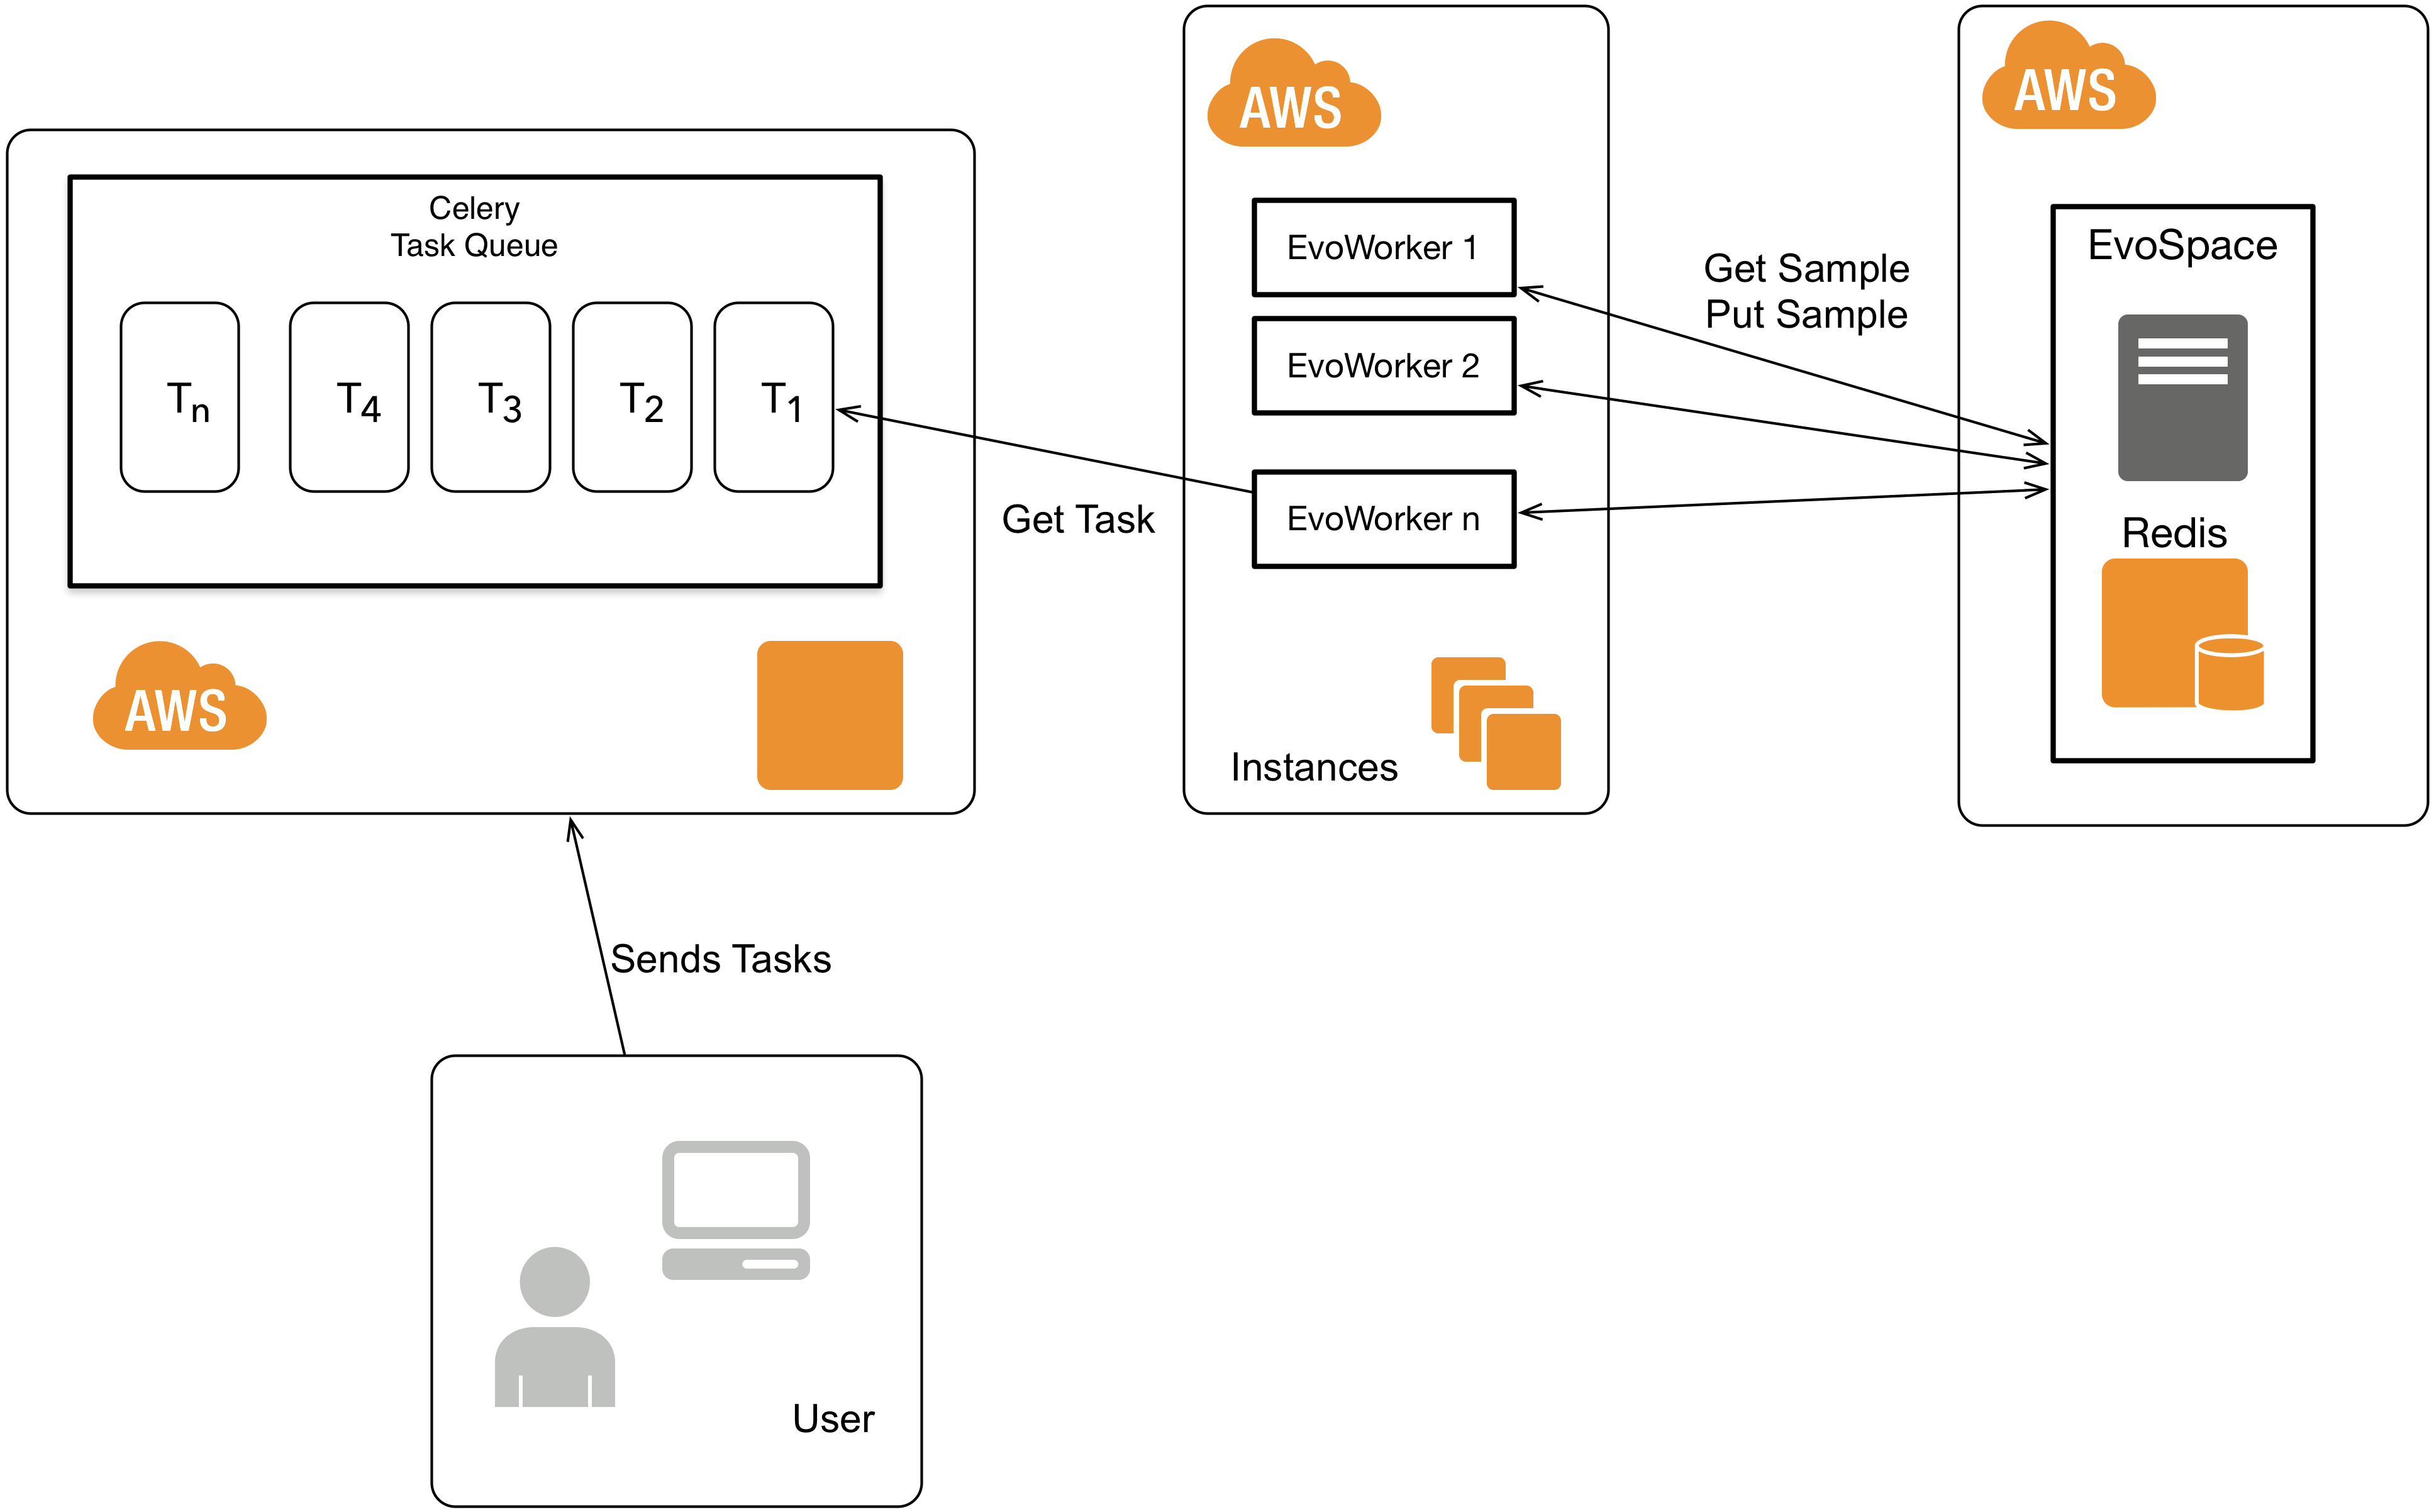
\includegraphics[width=9cm]{img/EvoSpaceAWS.png}
    \caption{Figure showing the elements of the cloud implementation of EvoSpace, and what are the relationships between them. The right-most component holds the {\em pool} from which EvoWorkers (in the middle) extract elements to evaluate, and where results are put back.}
    \label{fig:evospace}
  \end{figure}
%
\section{EvoSpace Cloud Implementation}
\label{sec:evo}

The EvoSpace framework, which was introduced in \cite{Evospace}, and
since then used in different applications
\cite{GValdez2015,garcia2017evospace}, is functionally divided in two
parts, which are also shown in Figure \ref{fig:evospace}, the EvoSpace
{\em pool}, with the evolving population that is decoupled from the
workers, which we call EvoWorkers, and are the ones actually
performing the evolutionary process transiently on the population,
whose origin and destination always is the EvoSpace Pool.

In a basic EvoSpace configuration, a certain number of EvoWorkers request a small random sample of the
population, the size of this sample is specified by the {\em Population Size} parameter (see Table \ref{tab:params}).
Using this sample as the initial seed for a local EA executed
on the clients, containers or cloud instances;  in this case, we implemented the 
local EA of each worker using the DEAP Python
library \cite{fortin2012deap} using the following parameters: For OneMax, two-point crossover,
tournament selection, tournament size=4, and bit-flip mutation.  We used
Gaussian mutation for continuous functions with $\mu=0$ and $\sigma=0.5$ and the
initial random values in the [-5,5] range. The number of generations and 
the number of times an EvoWorker takes a sample depend on the problem size,
these parameters are also reported in Table \ref{tab:params}. After the 
local EA finishes, EvoWorkers return the evolved population back to the pool.

The experimental platform used in this work is
described in \cite{valenzuela2015implementing}, and consists of different virtual machines
created automatically by a script before each experiment.

Each experiment consists of the following steps:

\begin{enumerate}
    \item First, the script creates two virtual machines: one for the task queue and another
    for the EvoSpace container. Then it creates the number of worker machines needed, these
    machines are configured as client machines for the task queue.
    \item For each run the number of EvoWorkers needed are added to the queue as tasks, from
    the user's PC.
    \item Every worker machine loads the task and the experiment
      starts. During the experiment every worker takes from and replaces
      samples in the EvoSpace container.
    \item Finally, all the data generated in each workers is returned by the task queue.
    \end{enumerate}

This setup was deployed on top of the Amazon Web Services (AWS)
platform which allowed the execution of the experiments with similar computing resources.

\section{Experiments}
 \label{sec:experiments}

\begin{table}[!t]
\caption{Ranges for EvoWorker parameters used in the OneMax benchmark}
\label{tab:params}
\centering
\begin{tabular}{l|cccccc }
\hline
\textbf{Parameter} & \multicolumn{3}{c}{OneMax} & \multicolumn{3}{c}{Test Functions} \\
\hline
Number of Workers & 2 & 6 & 12 & 2 & 6 & 12\\
\hline
\hline
Population Size & 200 & 280 & 620 & 120 & 150 & 150\\

Sample Size & 40 & 40 & 40 & 40 & 20 & 10\\

Maximum Samples & 30 & 40 & 40 & 200 & 100 & 50\\

Local Generations & 30 & 30 & 30 & 100 & 100 & 100\\

\end{tabular}
\end{table}
%
The goal of this work is to provide more proof that a random static parametrization for each of the $n$ EvoWorkers
collaborating on a given run could achieve competitive results against an homogeneous tuned parametrization
\cite{fuku1,fuku2,LNCS86720702}. The parameters considered to be randomly set for each EvoWorker
were the crossover and mutation probabilities, with a valid range of $[0,1]$. These parameters were
selected because they effectively control which types of moves in the search space are
applied, and are related to the amount of exploration and exploitation
that is carried out.
The other parameters and design choices used by EvoSpace and the EvoWorkers in our experiments are given in
Table \ref{tab:params}. Additionally, for the binary OneMax problem bit-flip mutation
is used with an independent probability for each attribute to be flipped (indpb) of $0.05$,
a two point crossover and a tournament selection of size 3. For the real-valued problems a Gaussian
mutation was applied with $\mu=0$, $\sigma=0.2$, and indpb=$0.05$; two point crossover and
a tournament selection of three. These values are kept static to measure only the effect of the
parameters mentioned above.

We are going to measure the effectiveness of RPW in EvoSpace by
comparing two parametrization strategies,
similar to what is done in \cite{fuku1,fuku2,LNCS86720702}. First, we consider the approach of setting all
of the EvoWorker parameters homogeneously. In order to tune the homogeneous parameters,
we select the best configuration from 100 random parametrizations.
Each of these random parametrization are evaluated based on their average performance over 10
independent runs for each problem.
Hereafter, we refer to this method as the {\em homogeneous} configuration.
Second, for RPW the parametrizations
are not tuned, every EvoWorker sets them independently and randomly at the beginning of each run.
Hereafter, we call this approach the {\em heterogeneous} configuration. Finally, we perform 30 independent runs
with both methods and report the average number of evaluations required by each strategy to find the
global optimum solution.

% I have moved this here to rearrange a bit graphics. This pushed down the whole thing.
\begin{figure*}[h!tb]
    \centering
    \subfigure [2 workers]
    {
        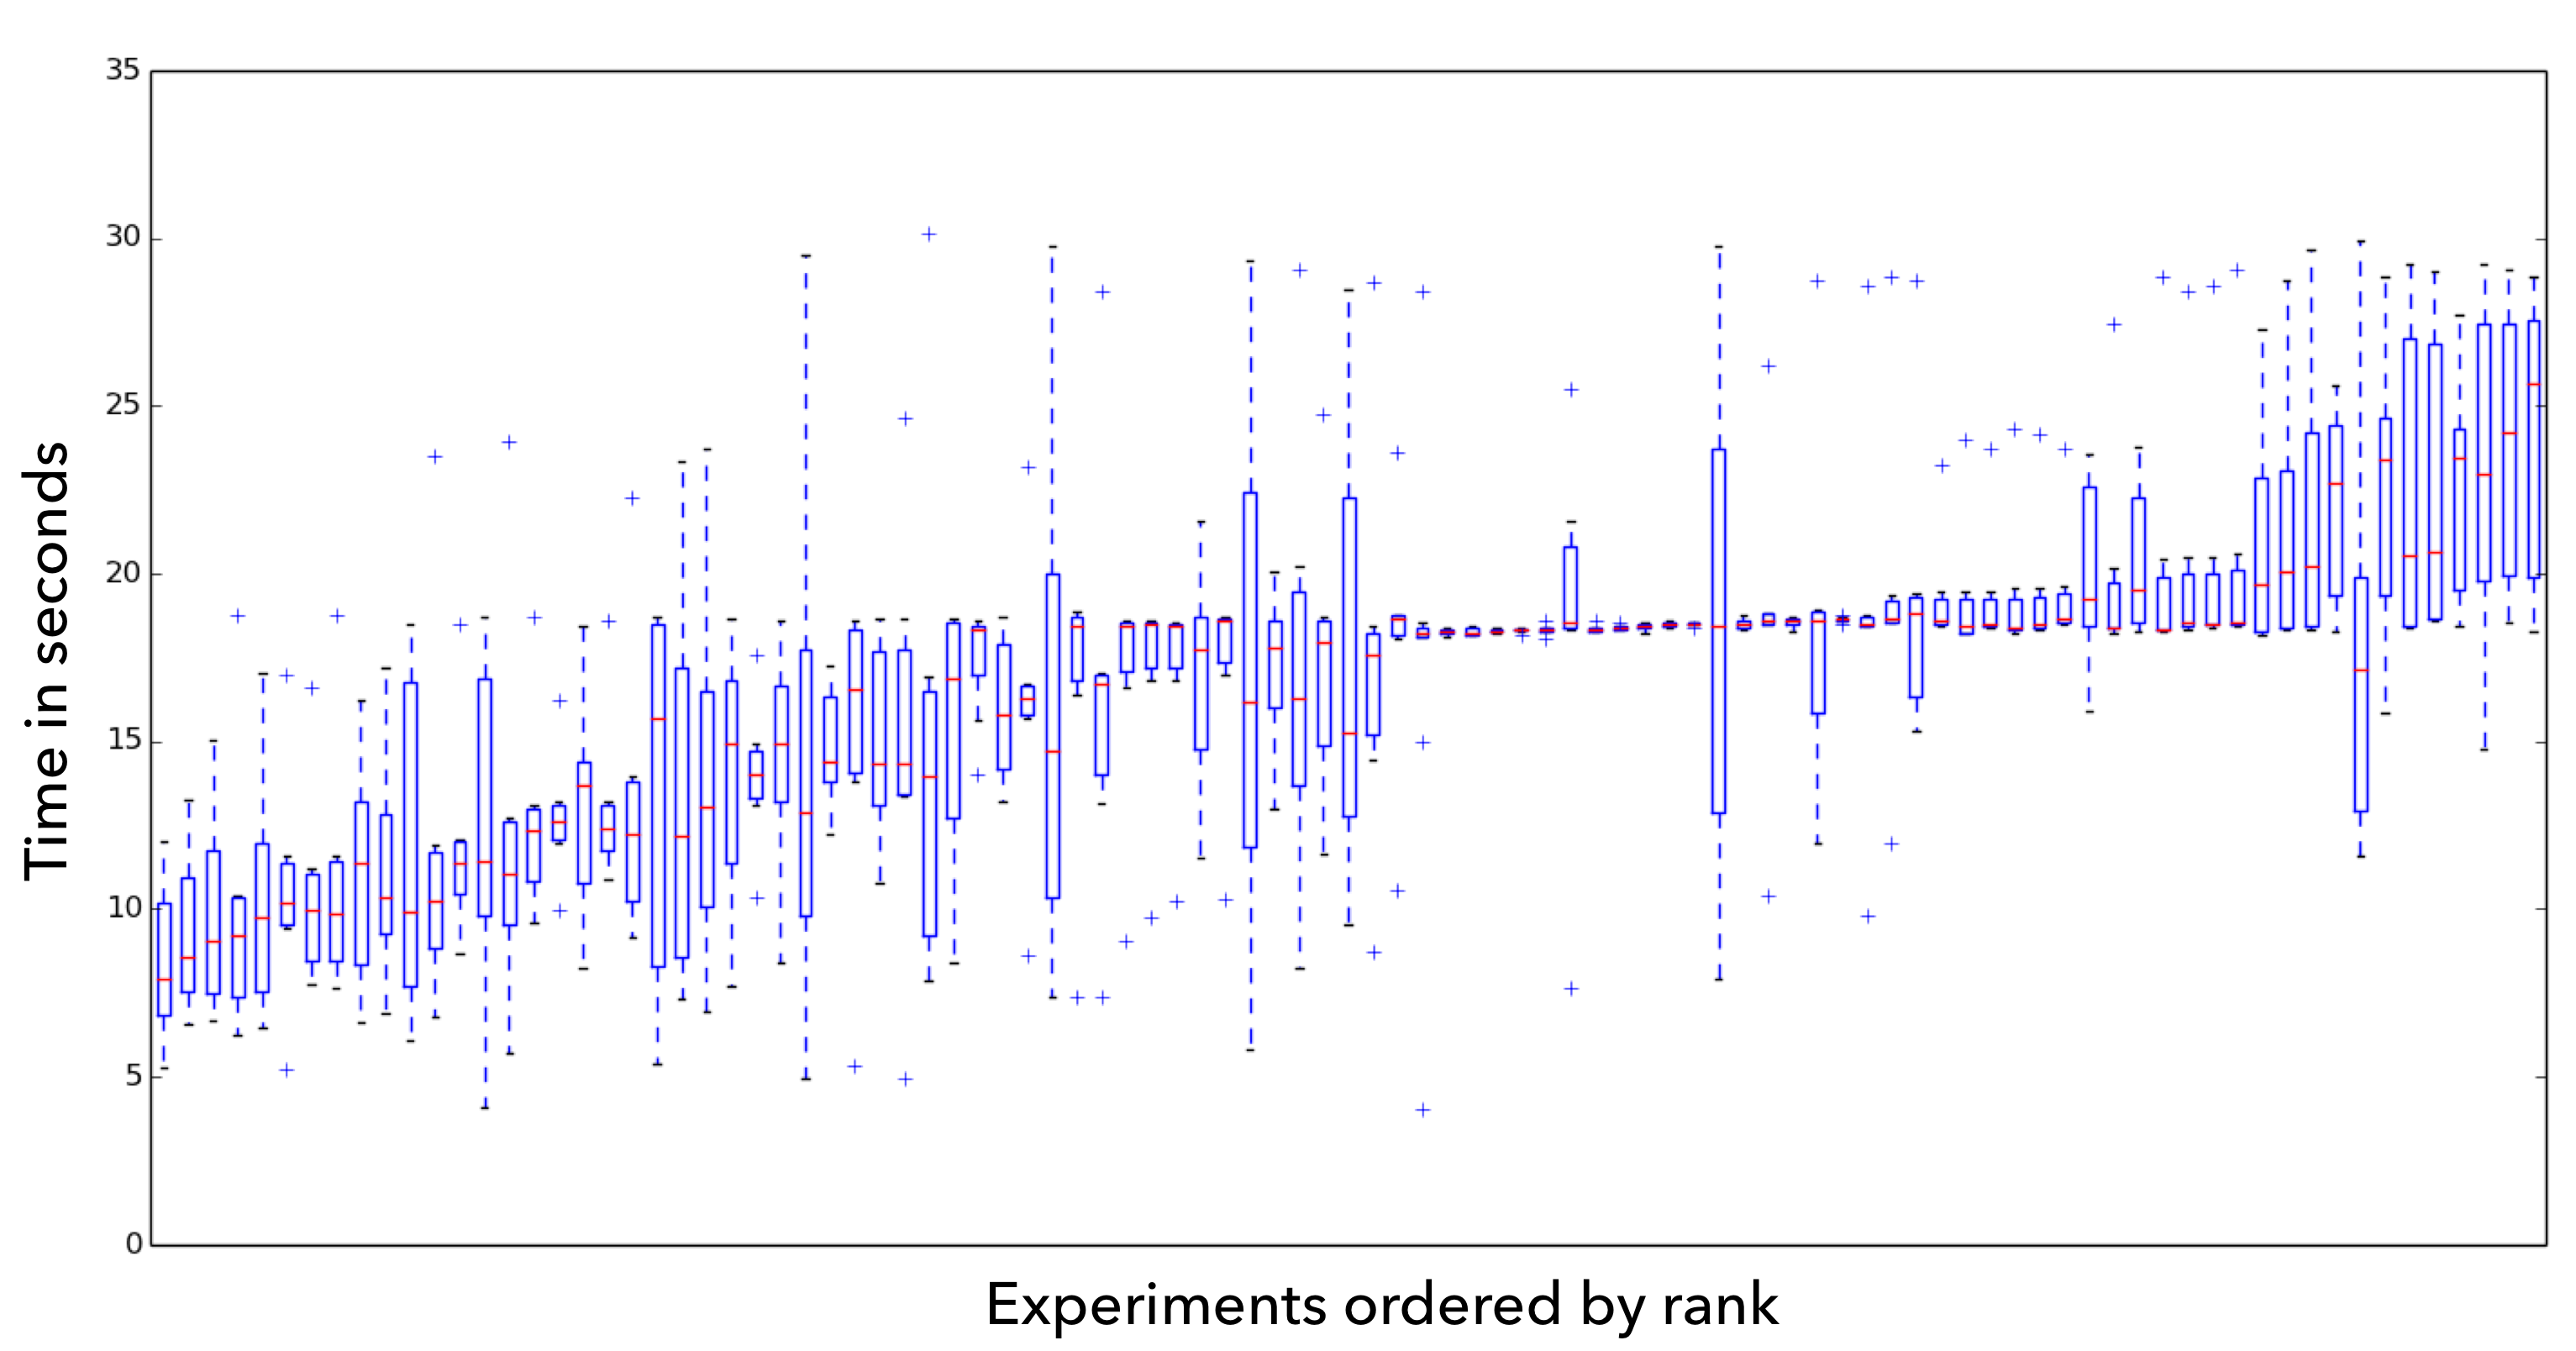
\includegraphics[width=4in]{img/2w_onemax_100_box.png}
    }
    \subfigure  [6 workers]
    {
        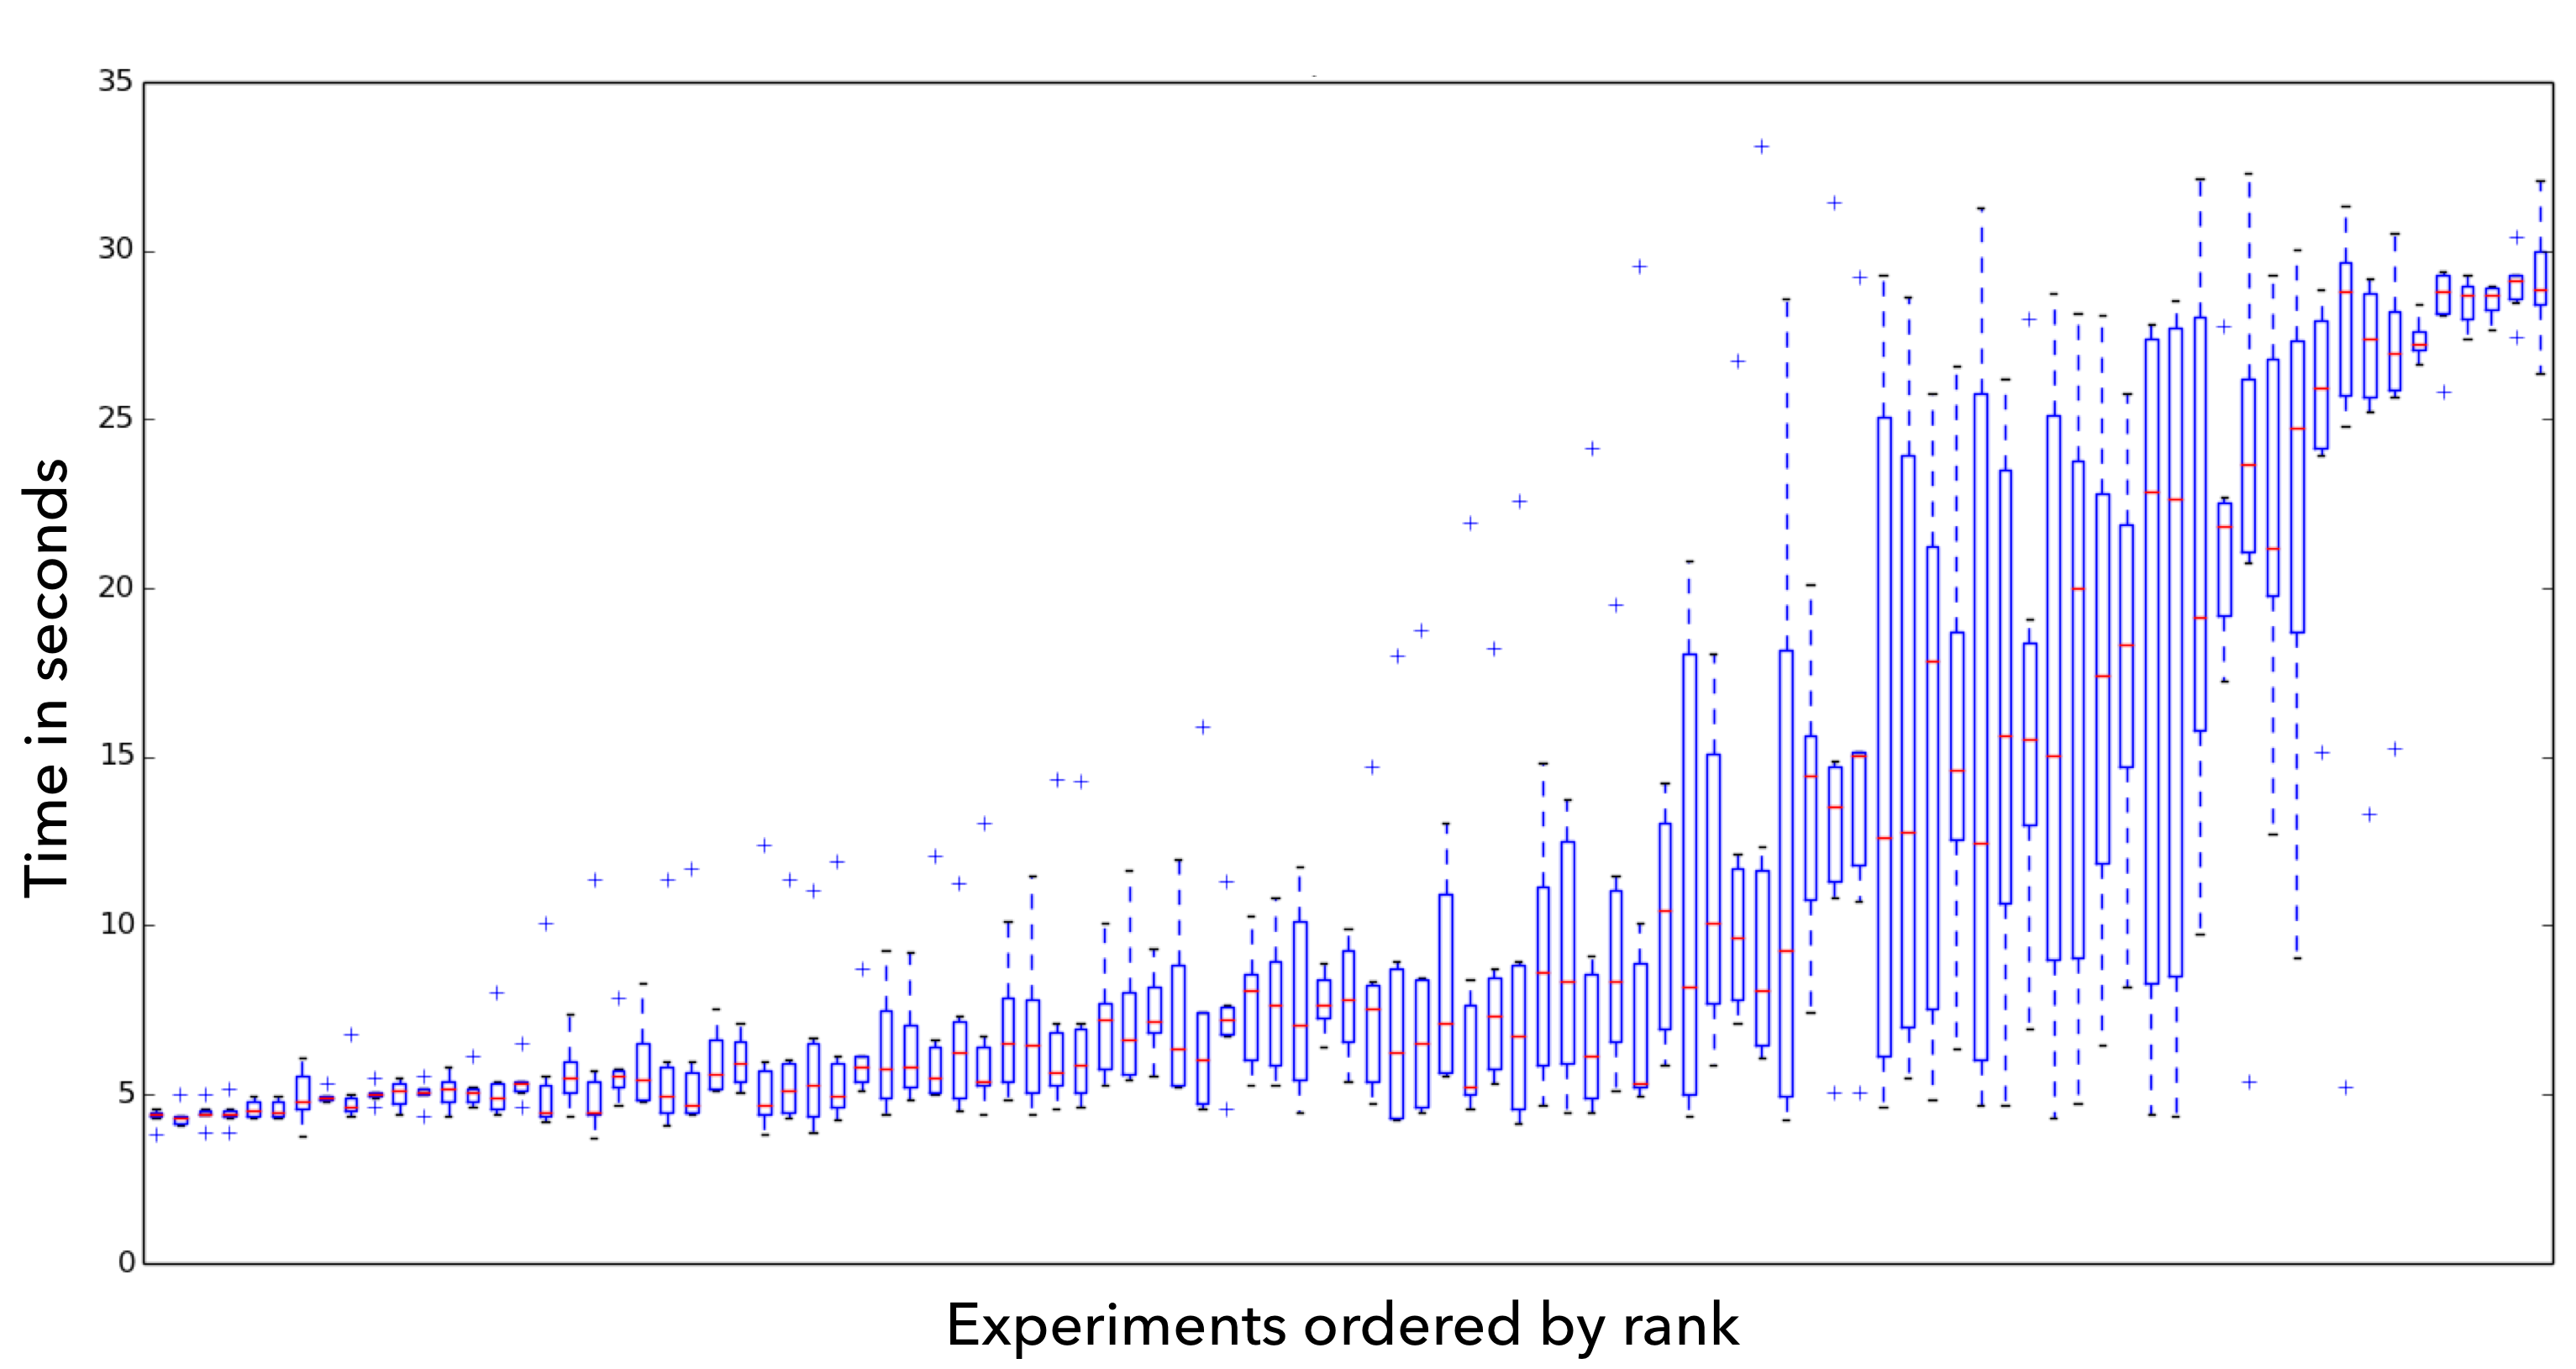
\includegraphics[width=4in]{img/6w_onemax_100_box.png}
    }
    \subfigure  [12 workers]
    {
        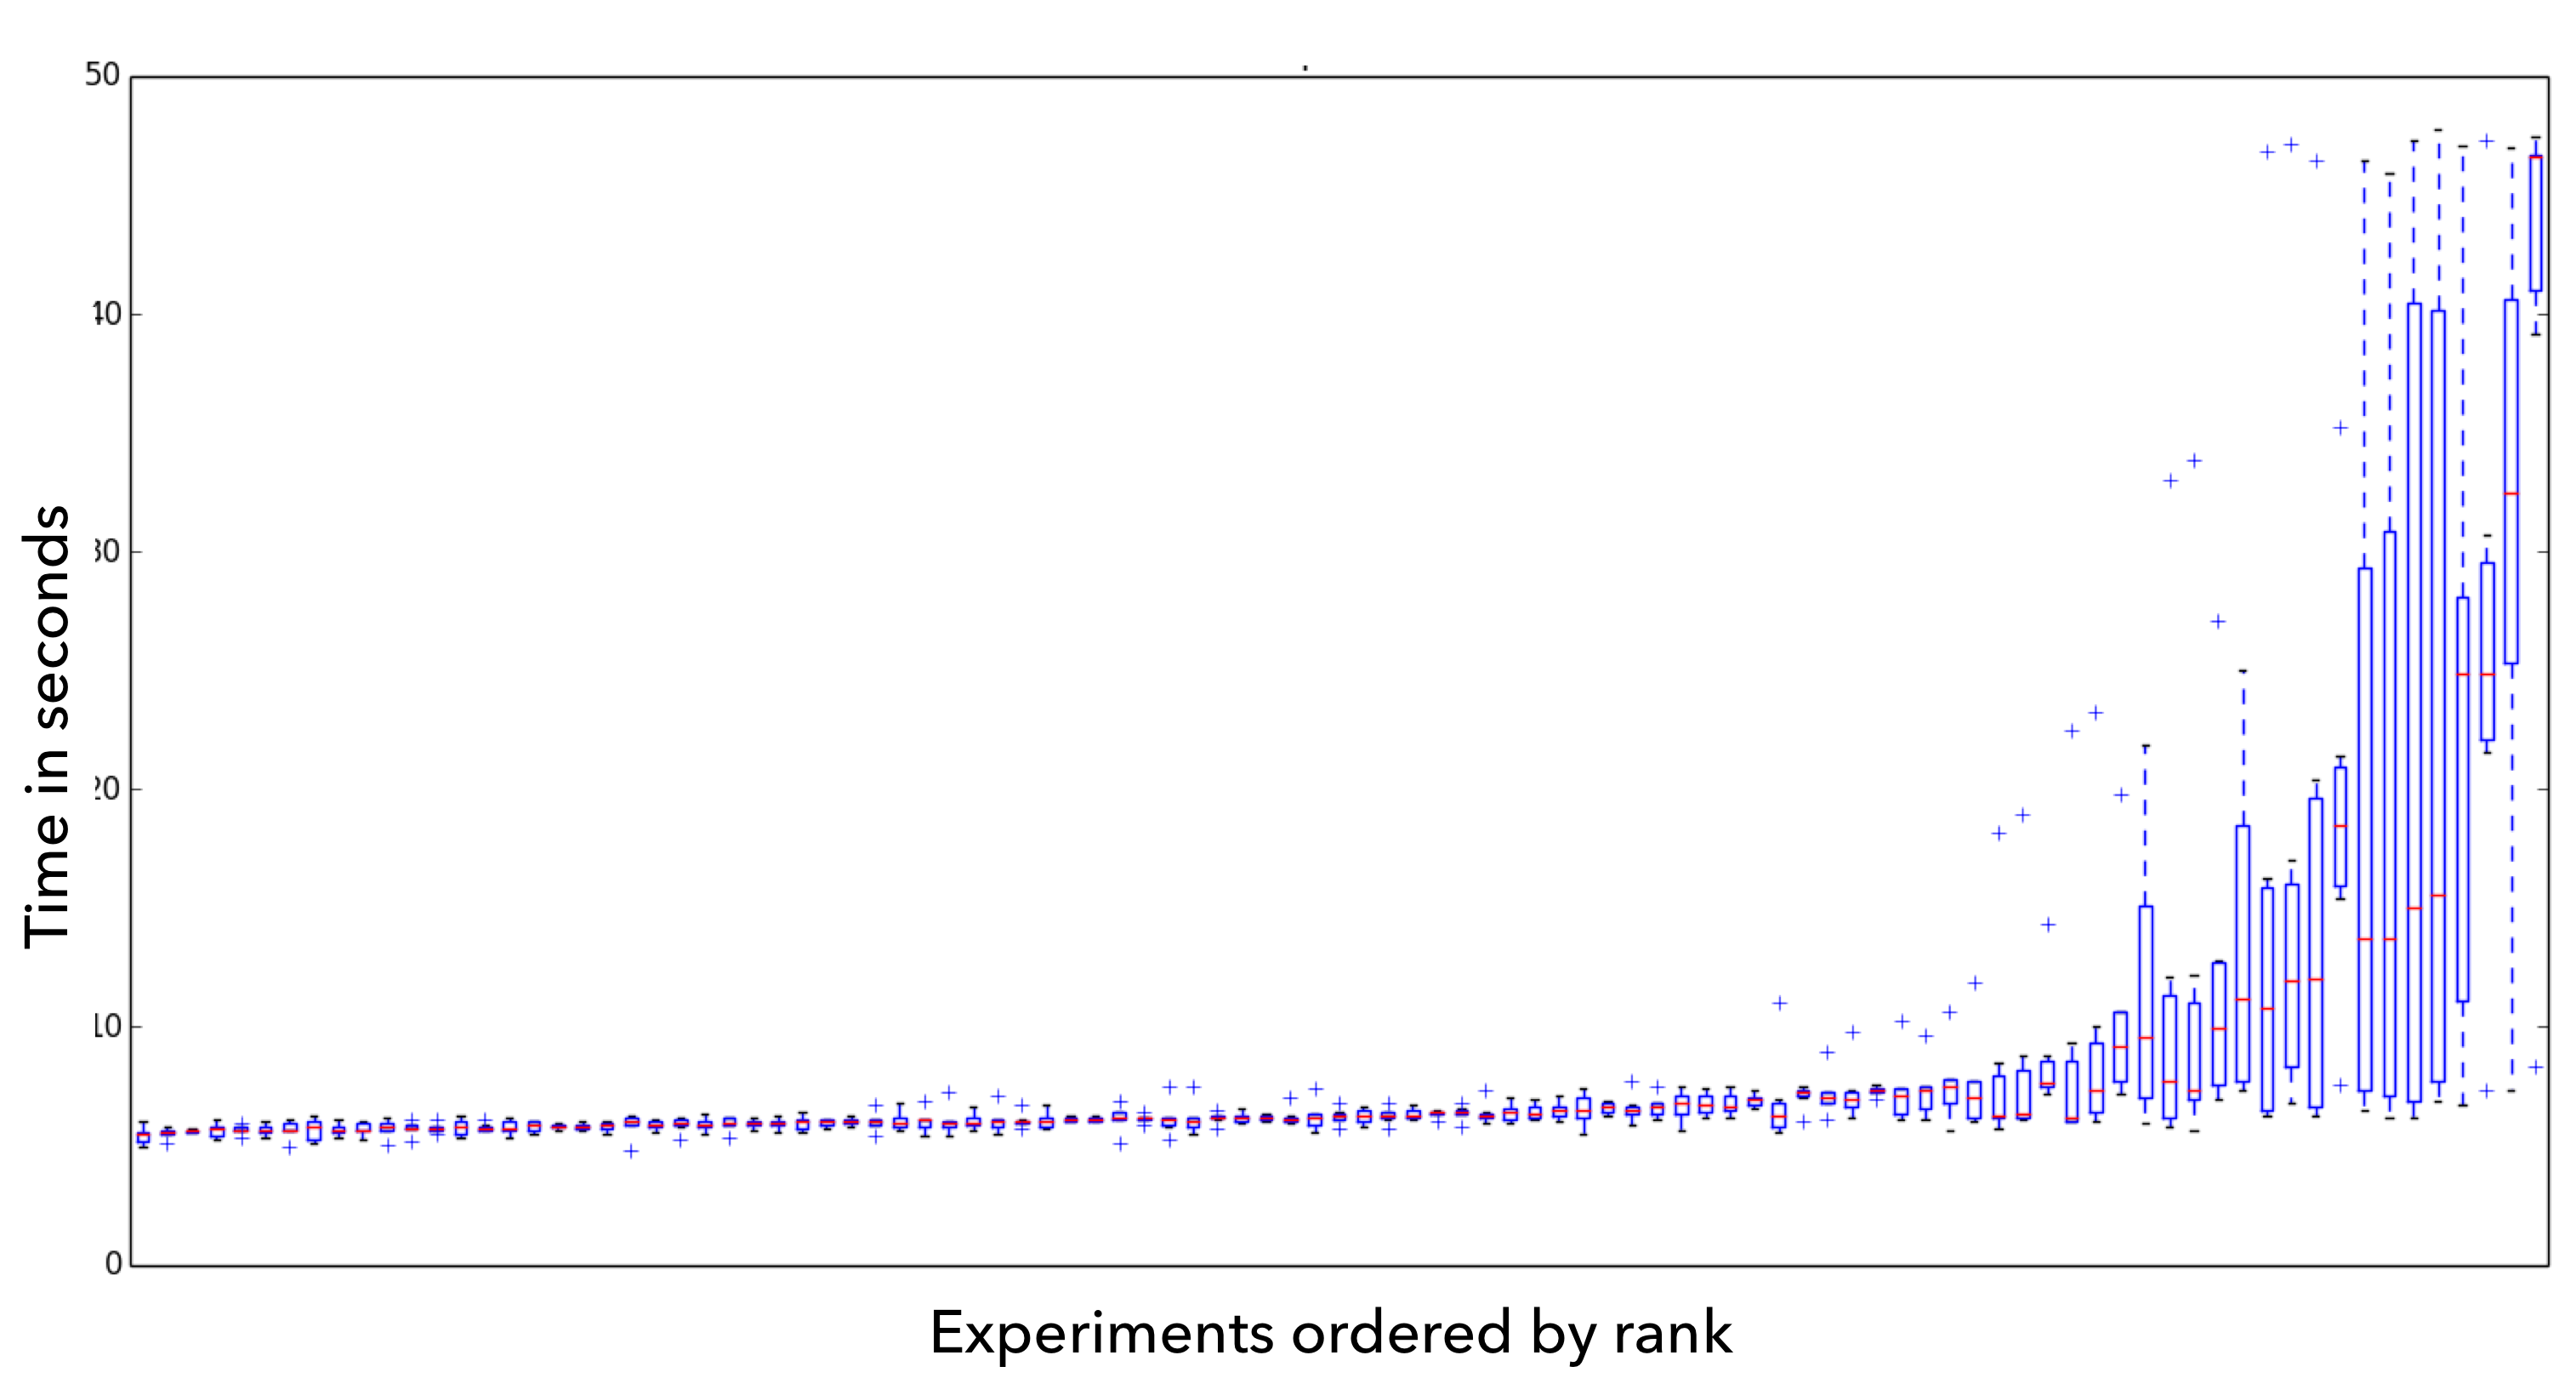
\includegraphics[width=4in]{img/12w_onemax_100_box.png}
    }

    \caption{100 experiments with random parameters for the 128 Bit OneMax problem.
    Experiments are ranked in increasing average time to solution
    order for 5 runs, with (a) 2 workers, (b) 6 workers, and (c) 12 workers.}
    \label{fig:effort}
  \end{figure*}
  %
The algorithms are first evaluated using the OneMax (or BitCounting) problem proposed by
Schaffer and Eshelman \cite{SE91}, this is a simple problem consisting in maximizing the number
of ones of a bitstring. Although the OneMax problem, by itself, may not justify the use of a distributed
implementation, i.e. we can argue that it can be solved in a very short time by using a
single desktop computer, it offers several advantages as a
benchmark for new architectures. It is a well-known problem with several
studies on parameters,  runtime analyses \cite{DBLP:journals/corr/MereloGVB15},
and distributed implementation
issues; and of course its difficulty will depend on the problem size. On the other hand, the drawback of using a benchmark that is not representative of
real-world problems is that experimental results may be only applicable to
problems similar to OneMax, where genetic operators are well suited for the
search in a solution space without deceptiveness or very large landscapes.
For the current experiments a 128 bit string was used. Since this
problem is not computationally demanding, more experiments were conducted for the tuning phase,
tuning the parameters using 2, 6, and 12 EvoWorkers. Then, following \cite{fuku1},
five standard real-valued single objective optimization problems were
tested: these are the Rastrigin, Griewank, De Jong, Schaffer  and
Ackley functions,
with the number of dimensions set to 100 in each case. For these problems we use a real-valued vector
representation for each individual.

  \begin{figure}[h!tb]
    \centering
        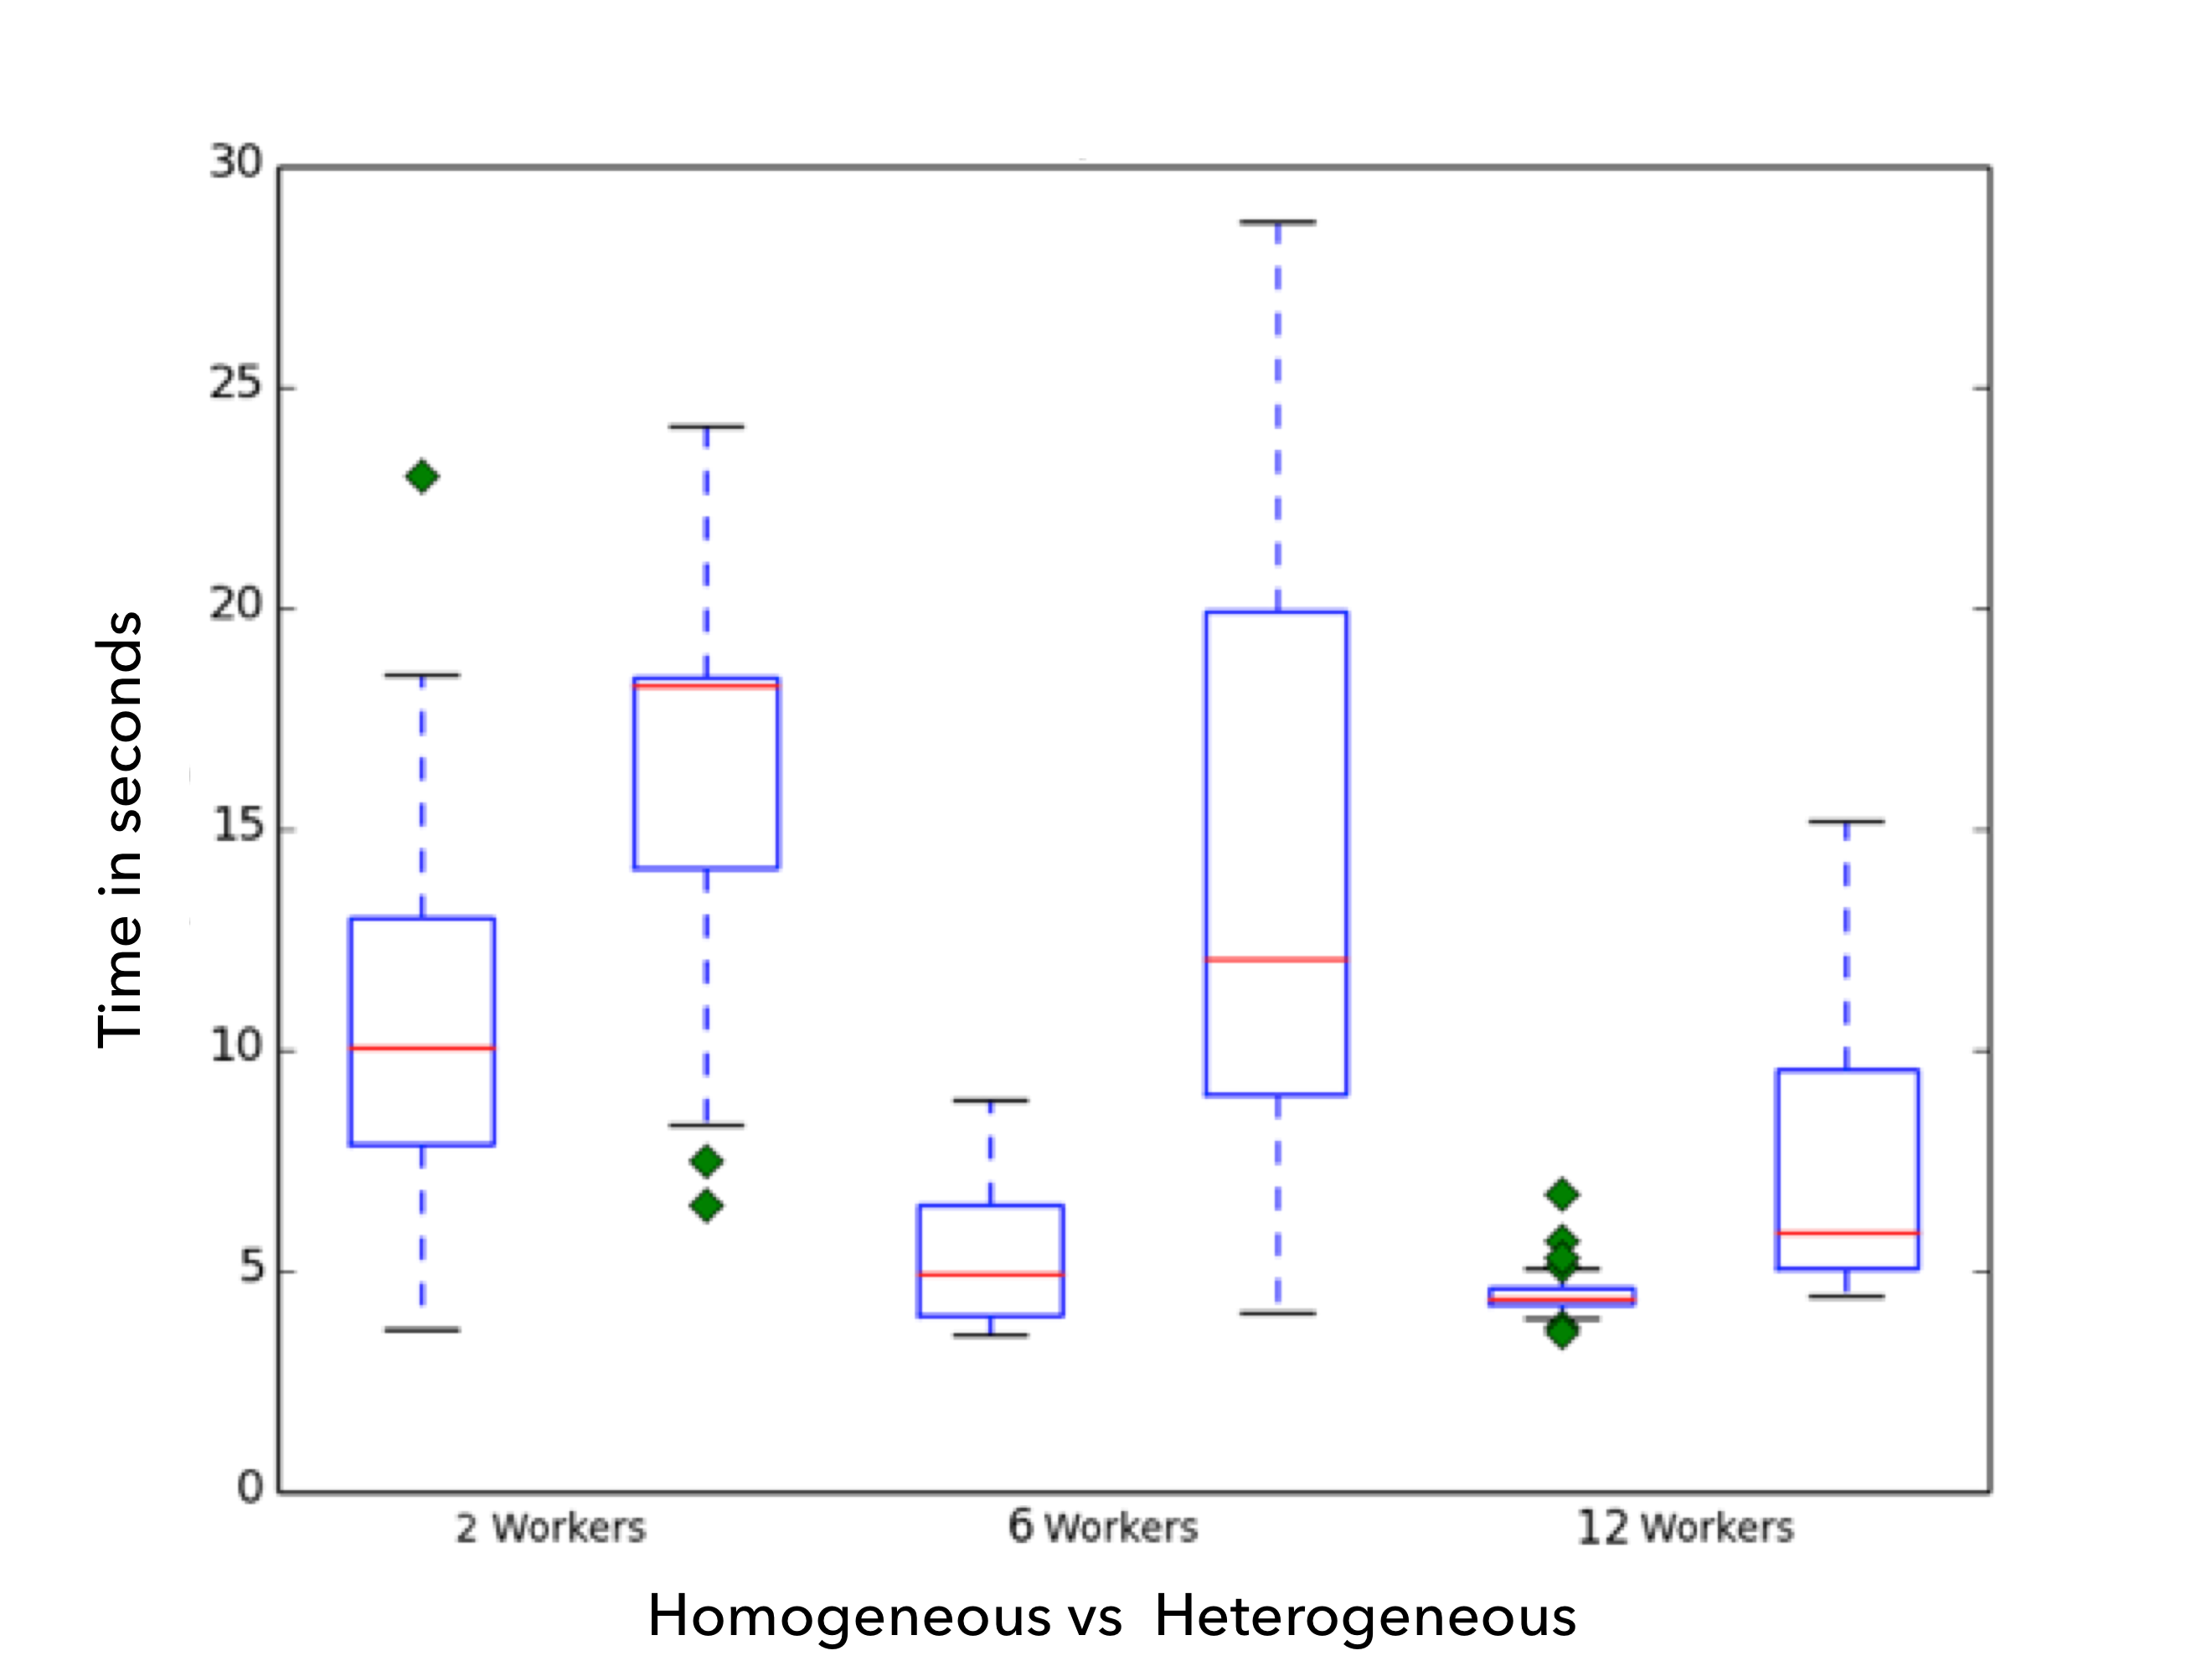
\includegraphics[width=9.5cm]{img/one_max_comp.png}
    \caption{Comparison of 30 runs of the 128 Bit OneMax problem.
    Box-plot of the time needed for solution, with homogeneus
    configurations using  2, 6 and 12 worker as a box-plot to the left of the $x$ axis
    tick, and heterogeneous configuration to the right. Outliers are
    shown as green rhombs.
    }
    \label{fig:comp-onemax}
  \end{figure}
%
  \subsection{Results for OneMax}
  \label{ss:onemax}

As mentioned before, the first step is to simulate the manual tuning of the parameters
by running 100 experiments with random parameters and then selecting the best configuration,
using the median performance over 5 runs. Since the OneMax problem is solved by almost all
configurations, performance is determined by the time required to find
the optimal solution. Please note that this tuning is used as a
baseline for setting parameters in the homogeneous configuration, and
is not really a part of the RPW algorithm. % Please Mario check that
% this is correct - JJ

Figure~\ref{fig:effort} shows the time required for different numbers of EvoWorkers.
It can be observed that even with an homogeneous configuration, as the number of workers
increases, solutions are found faster on average, which is only to be expected; you can see how the
curve slope starts to increase farther to the right as the number of
worker increases; the median time needed to find the solution also decreases,
with around 75\% of the experiments finding the solution in the same
amount of time, around 5 seconds, as the bottom chart in the
aforementioned Figure shows. However, the maximum time needed to find
a solution is also greater than the base configuration; please note than the chart for 12
workers expands the $y$ axis up to 50 seconds.
%In general, the number of function
%evaluations increases with number of workers, also in every time
%unit. This implies that the selection of a good configuration could be
%found easier when using a higher number of workers, relative 
%to the total wall-clock time. % I don't understand this - JJ
% I think is not right, there is no relation between FEs and Easier Configuration 
% I will put the paragraph as a comment 

In \autoref{fig:comp-onemax} the results of 30 runs comparing against the RPW approach is shown.
It can be observed that as the number of EvoWorkers increases the median of the time decreases, but
in this case the best of the heterogeneous solutions (12 workers) is only better than the worst homogeneous
solution. In this case, the heterogeneous/random configuration
presented in this paper does not obtain better results than the
homogeneous configuration using the best parameters found by random
search. This problem, which is deceptively simple, actually depends
more on the exploitative part than the exploratory part. The
heterogeneous worker solution, however, seems to lean more on
exploration by keeping high diversity, something that might not be
actually needed during the last phases of the OneMax problem. This
might be also the case for other combinatorial optimization problem,
but checking the cases when that happens is left as future work.

\subsection{Results for Real-valued Optimization Functions}
%
\begin{figure*}[t]
    \centering
    \subfigure  [6 workers]
    {
        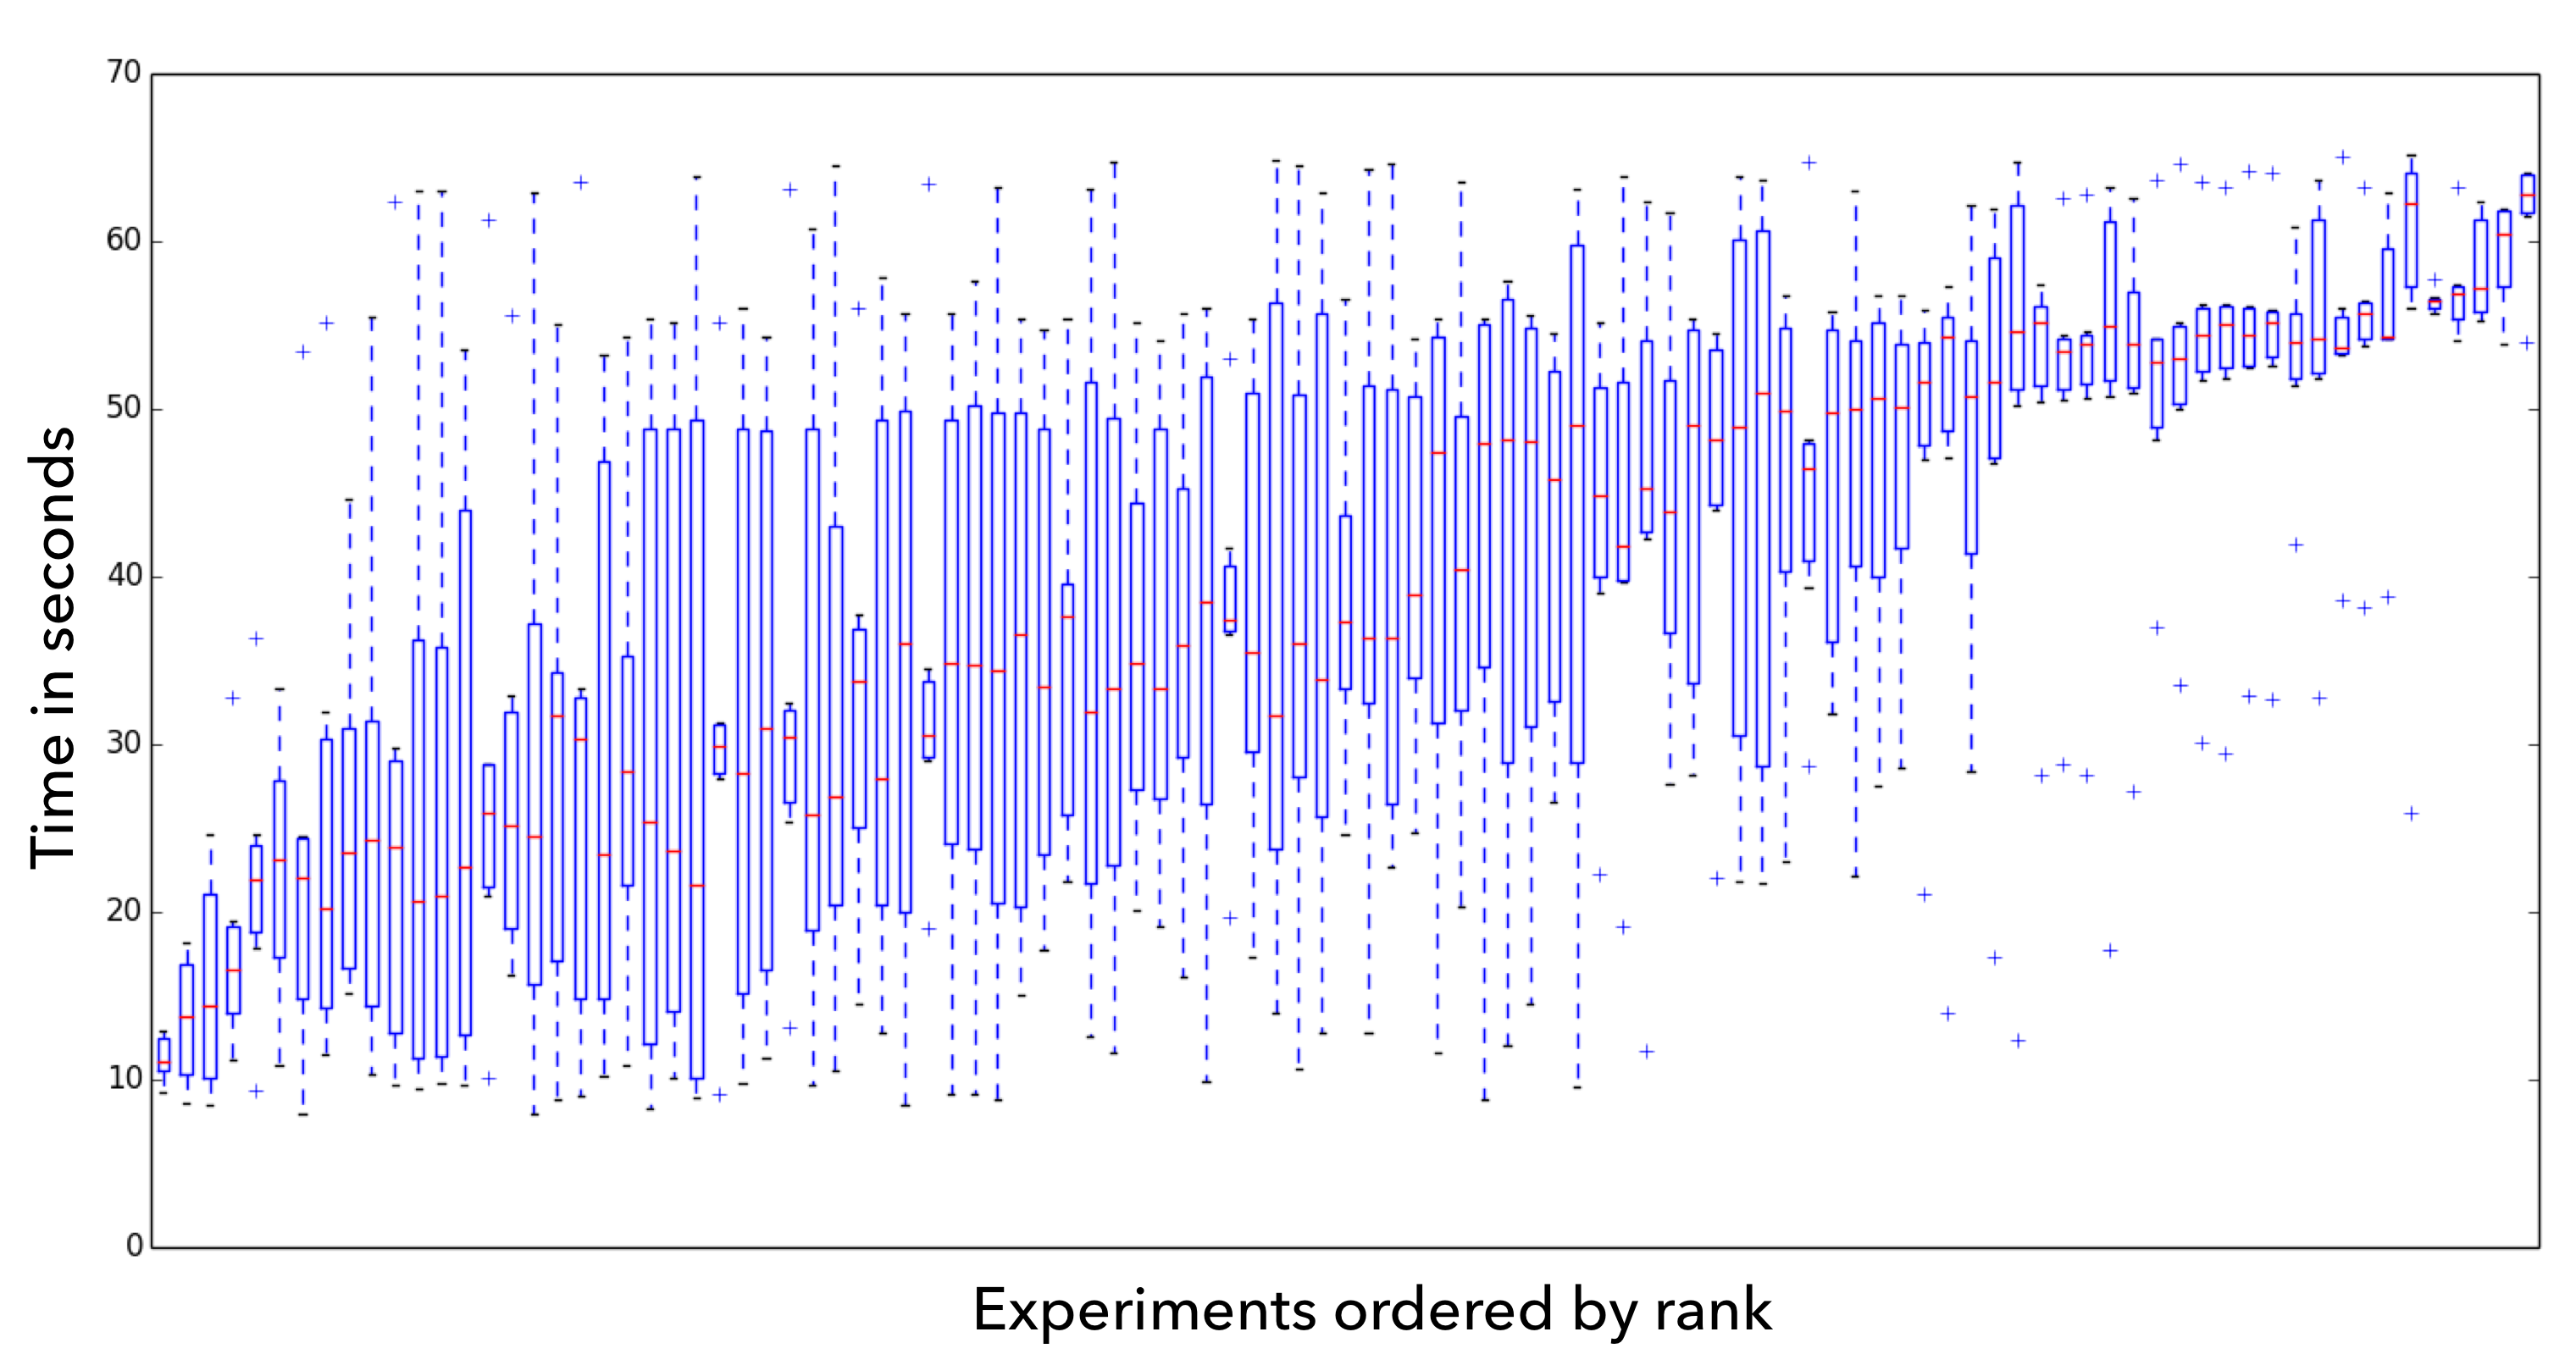
\includegraphics[width=3in]{img/6w_griewank_100_box.png}
    }
    \subfigure  [12 workers]
    {
        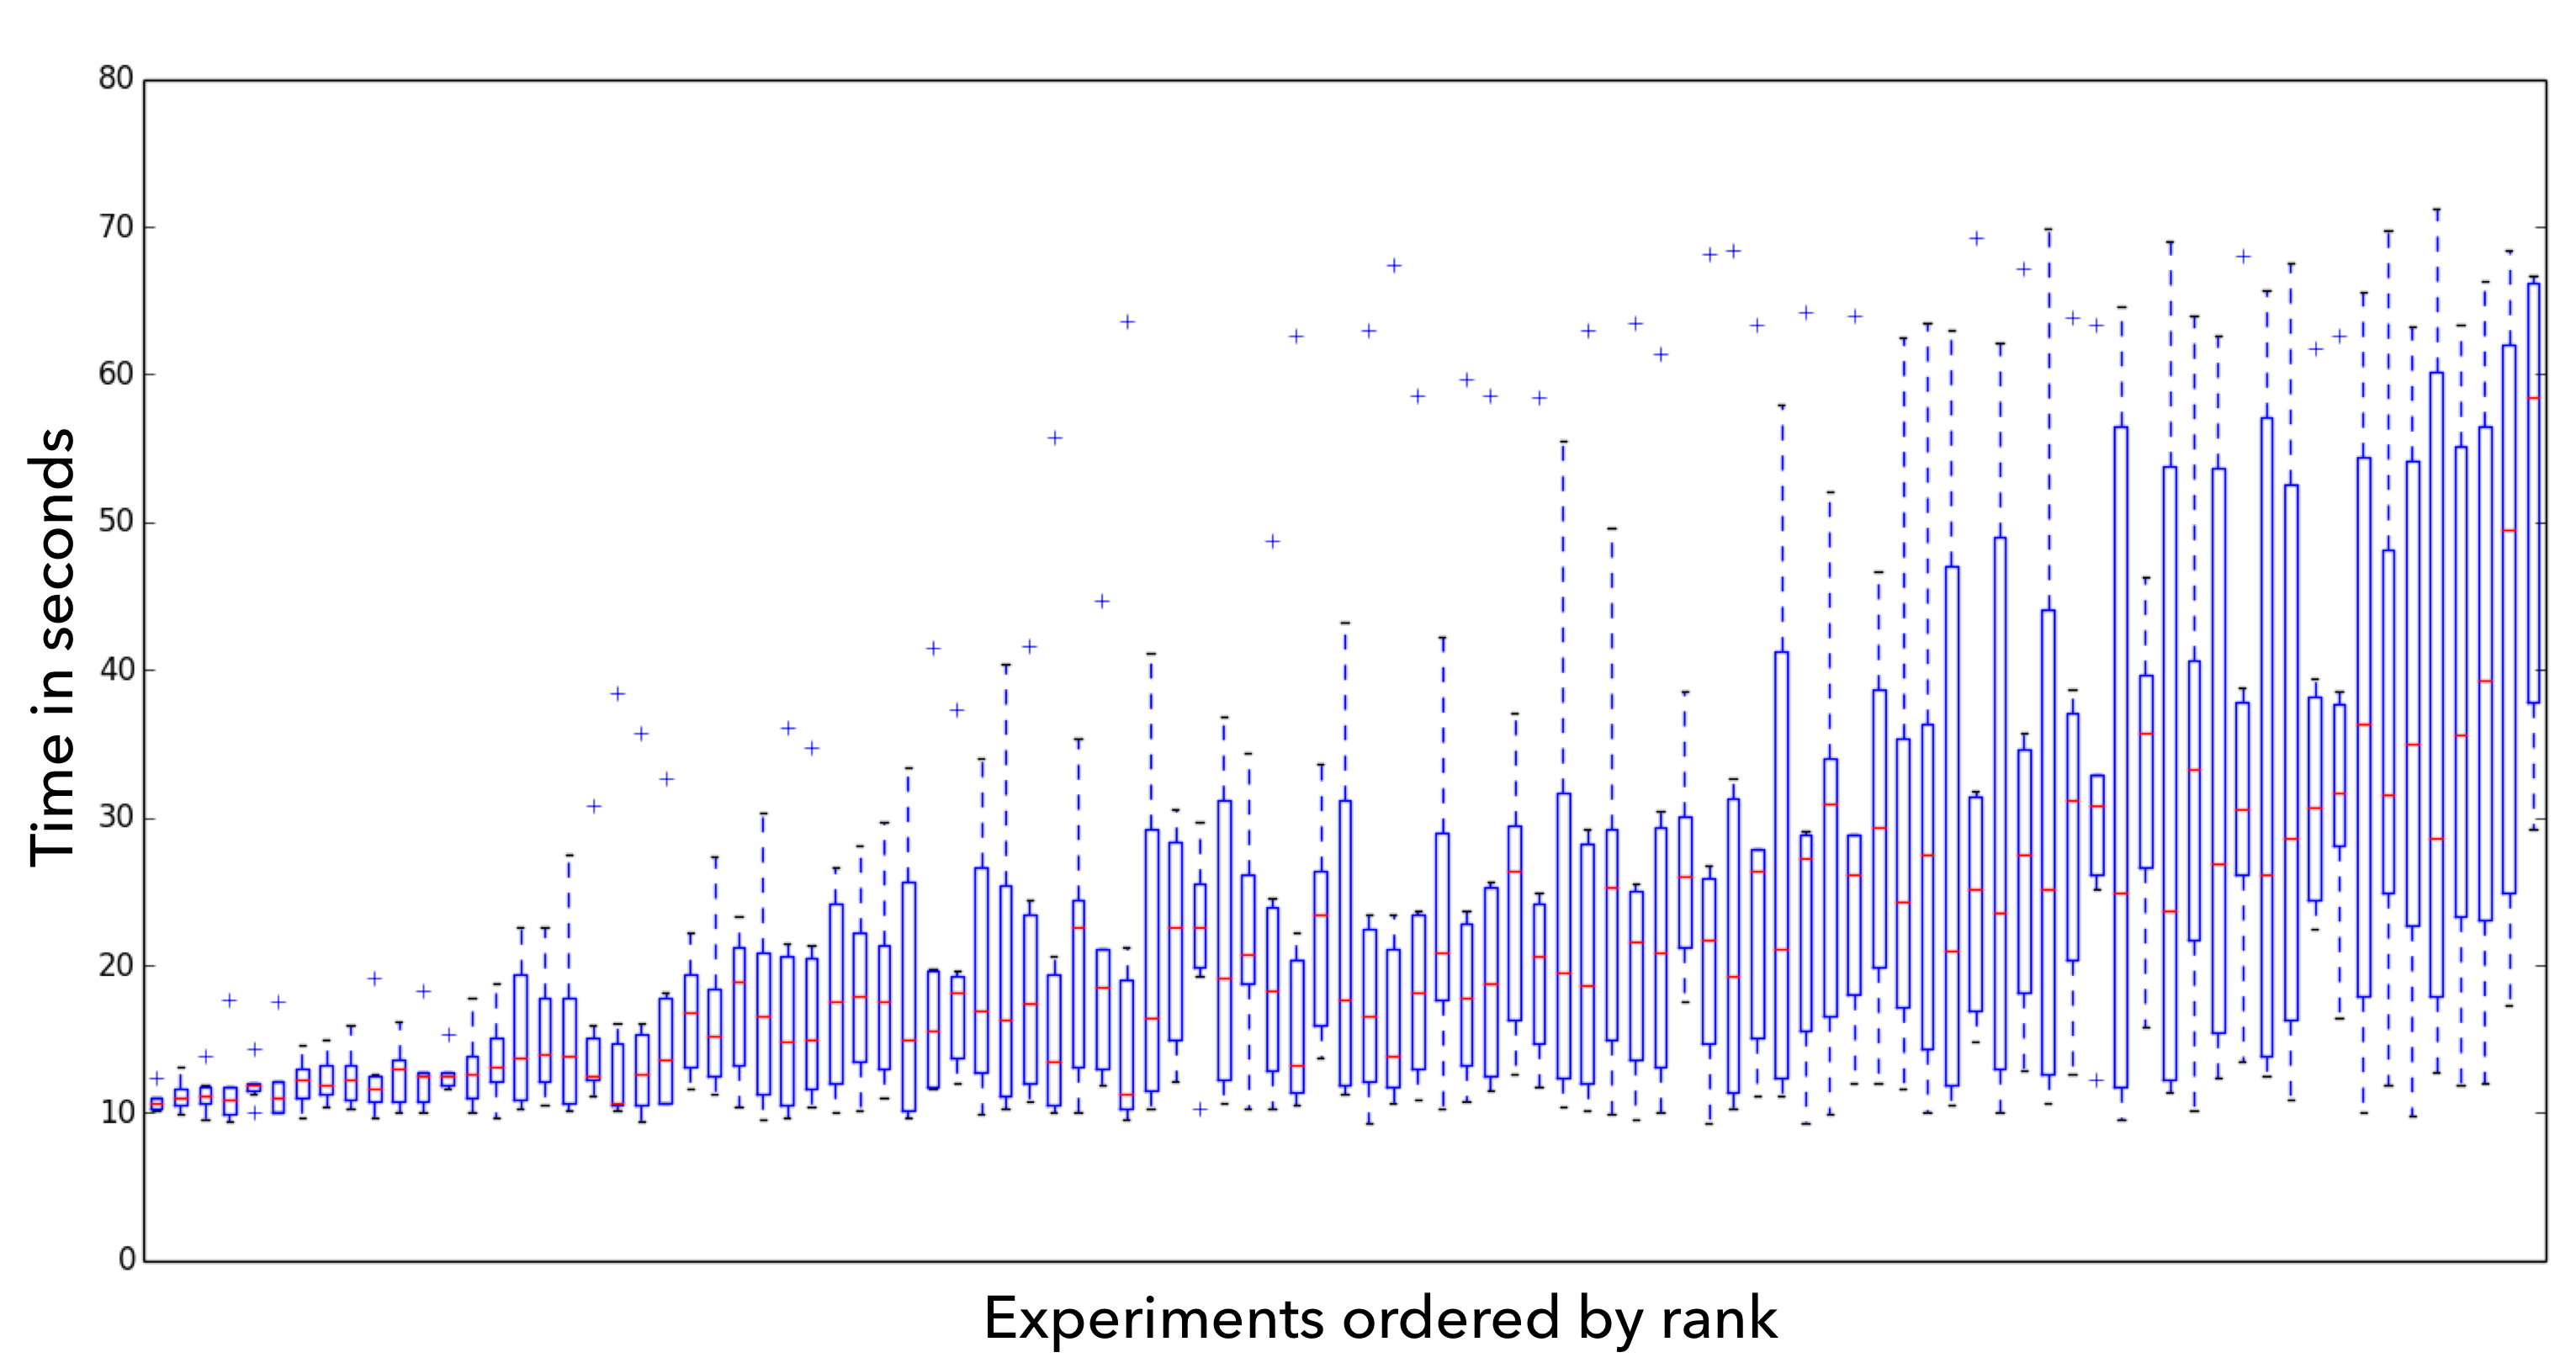
\includegraphics[width=3in]{img/12w_griewank_100_box.png}
    }

    \caption{100 experiments with random parameters for the 100 dimensions Griewank
    real-valued optimization test function. Experiments are ranked by
    the mean time to solution for 5 runs, with (a) 6 workers, and (b)
    12 workers. Please note that the scale of the $y$ axis is different.}
    \label{fig:griewank}
\end{figure*}
%
\begin{figure*}[t]
    \centering
    \subfigure  [Homogeneous]
    {
        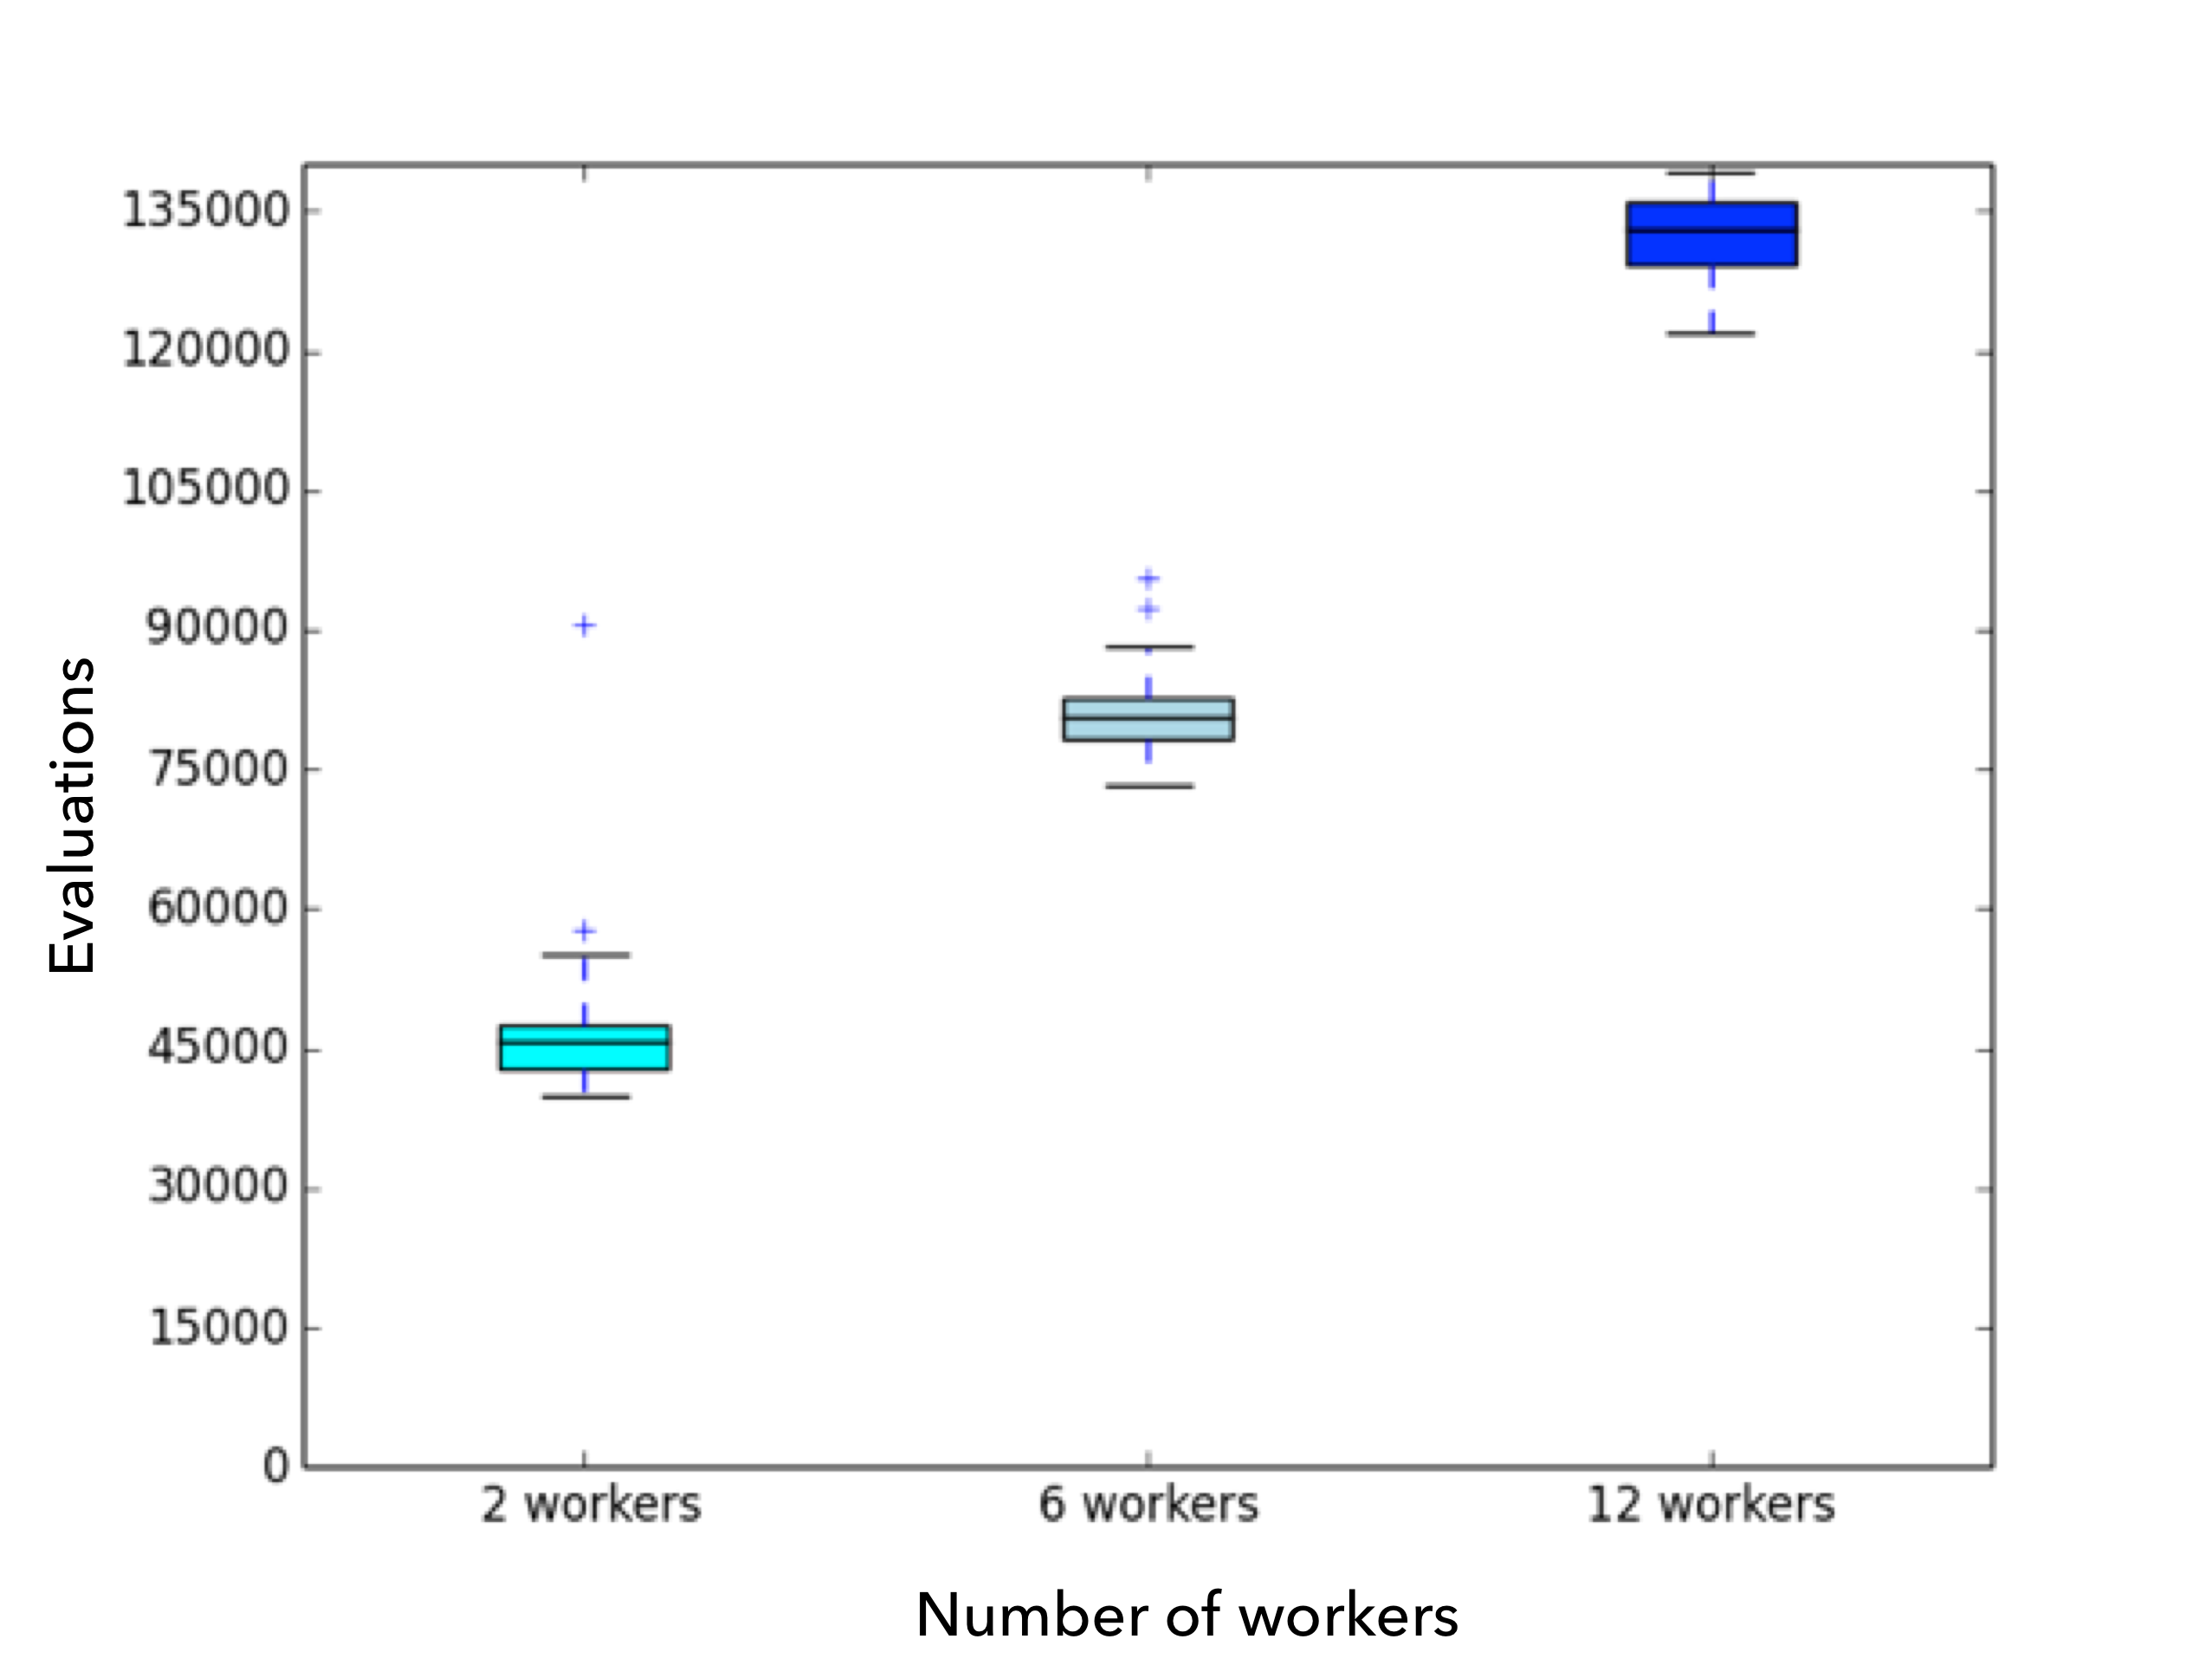
\includegraphics[width=3in]{img/griewank_evals_homo.png}
    }
    \subfigure  [Heterogeneous]
    {
        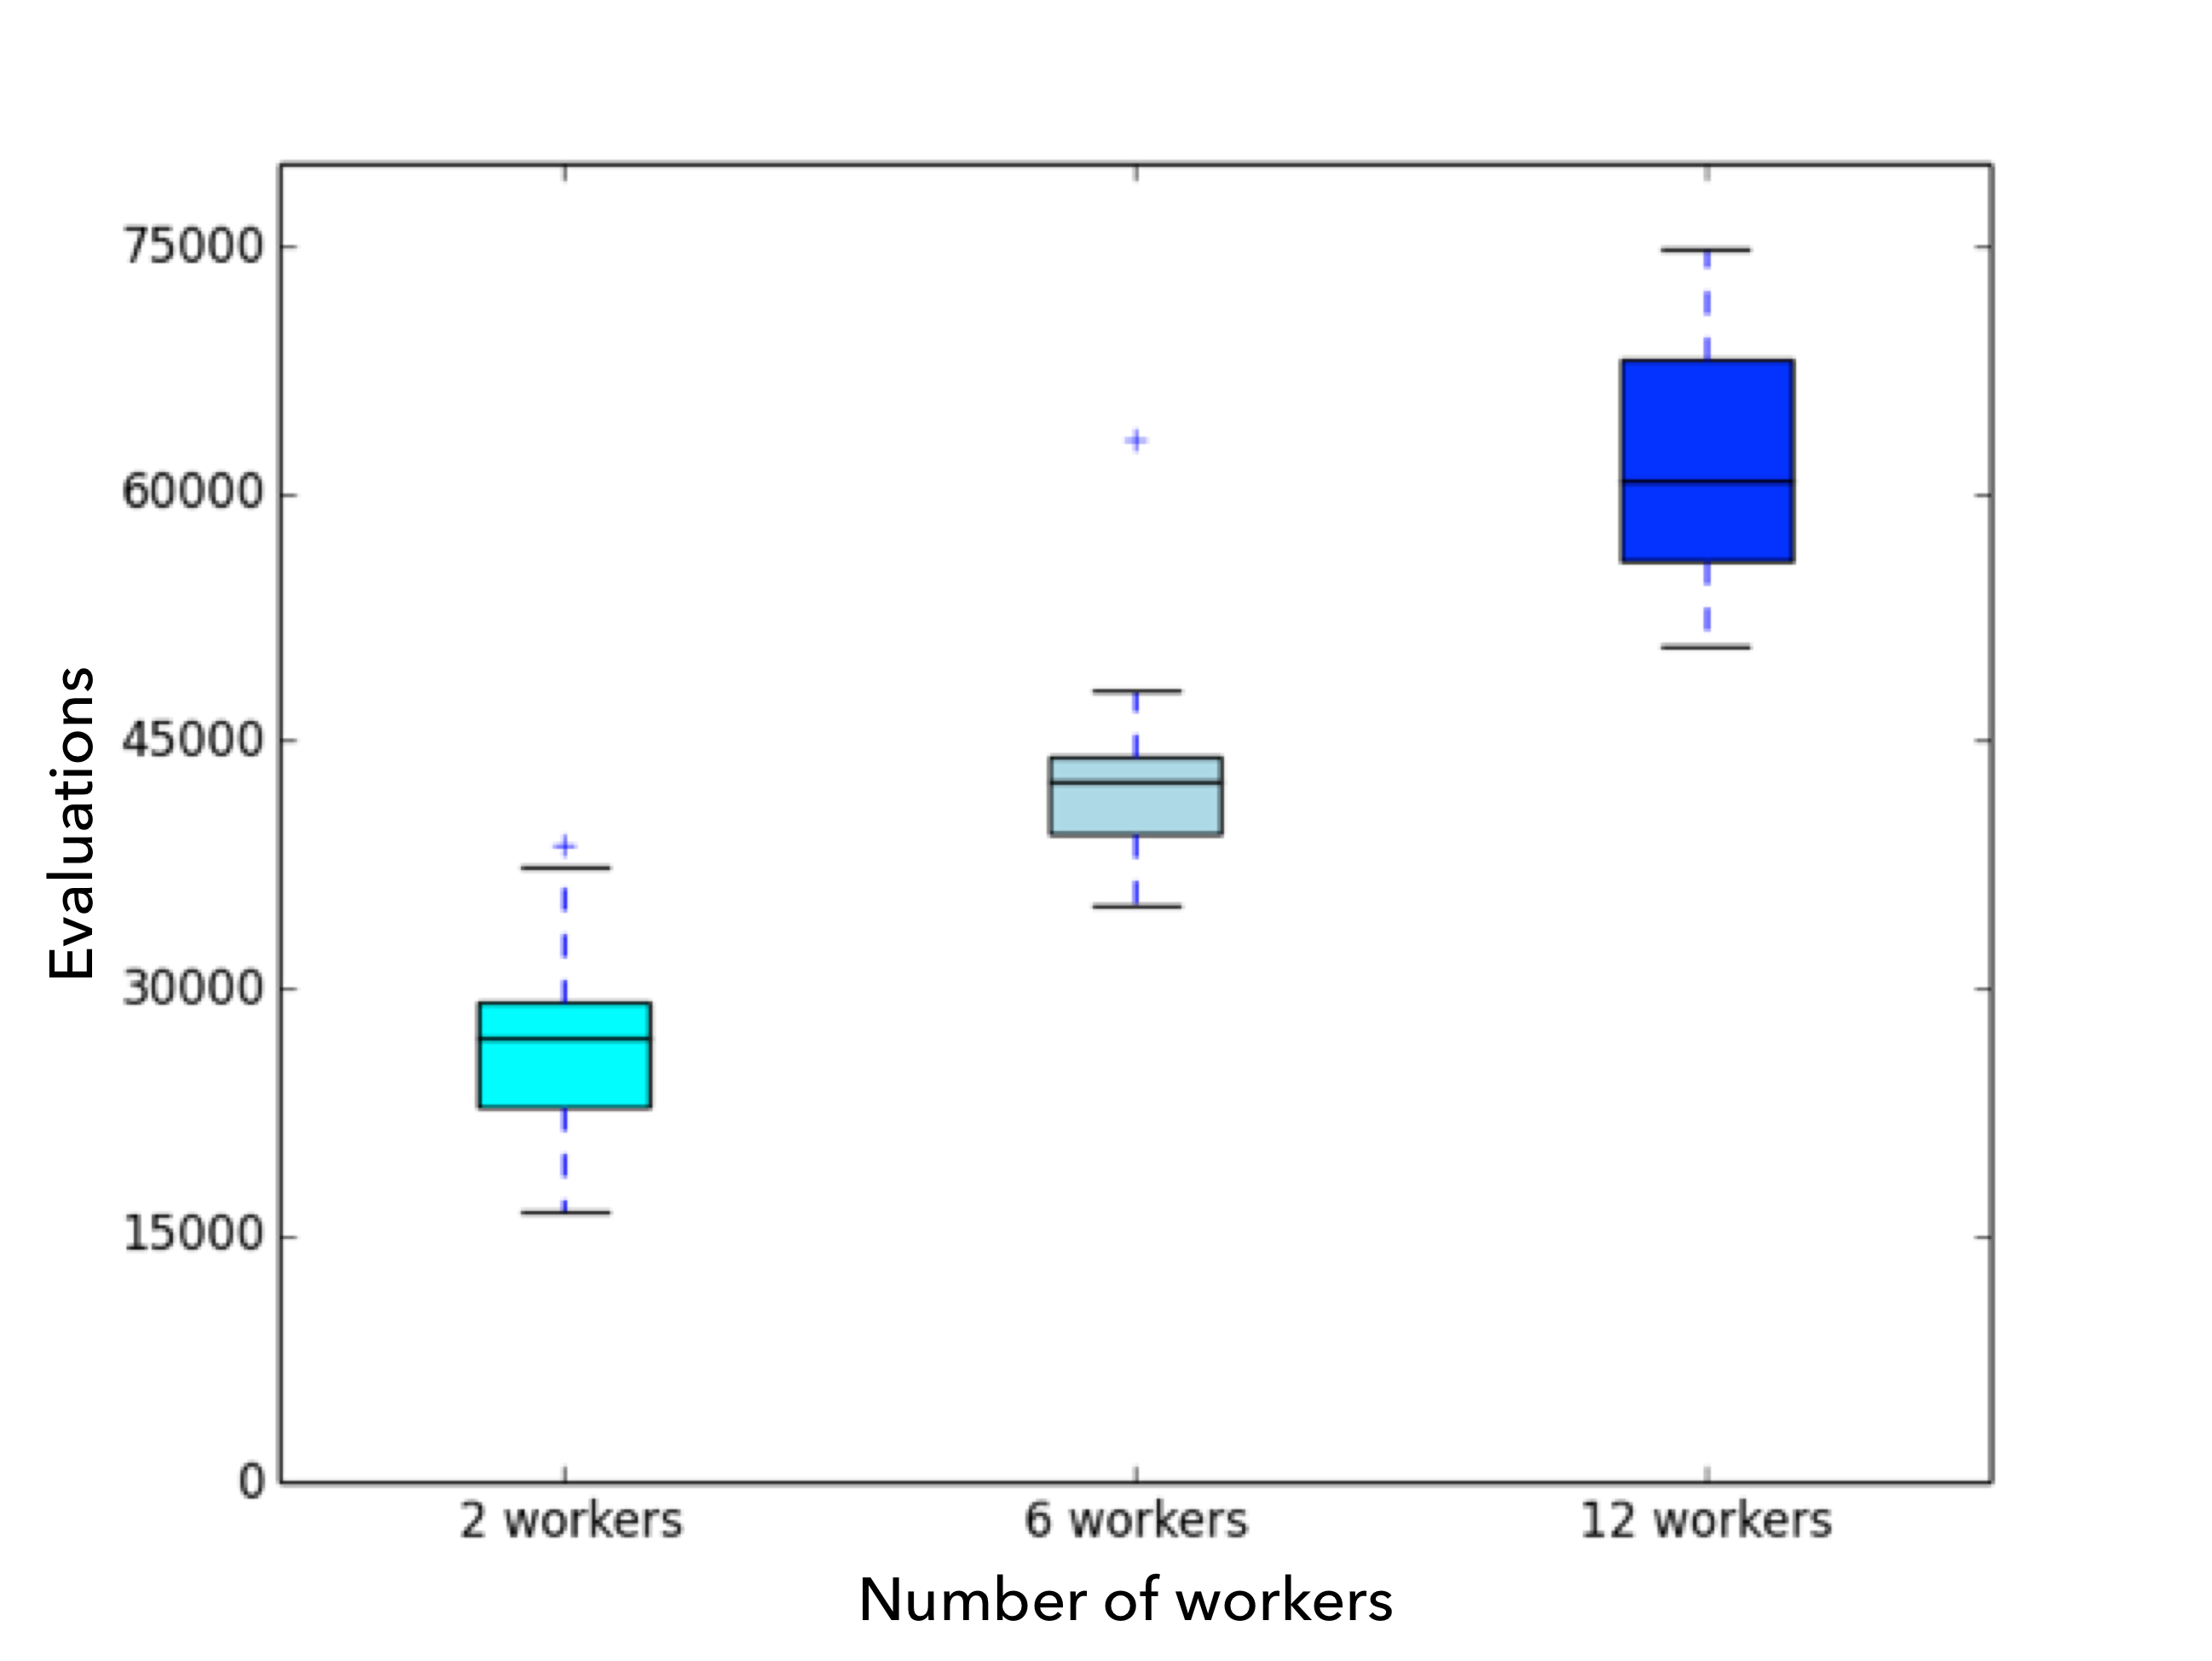
\includegraphics[width=3in]{img/griewank_evals_hetereo.png}
    }
      \caption{Box-plot of the
        evaluations used for the Griewank function by (a) Homogeneous configuration, and (b)
        Heterogeneous configuration. Please note that $y$ scales are different.}
    \label{fig:griewank-evals}
\end{figure*}
%
\begin{figure*}[t]
    \centering
    \subfigure  [Homogeneous]
    {
        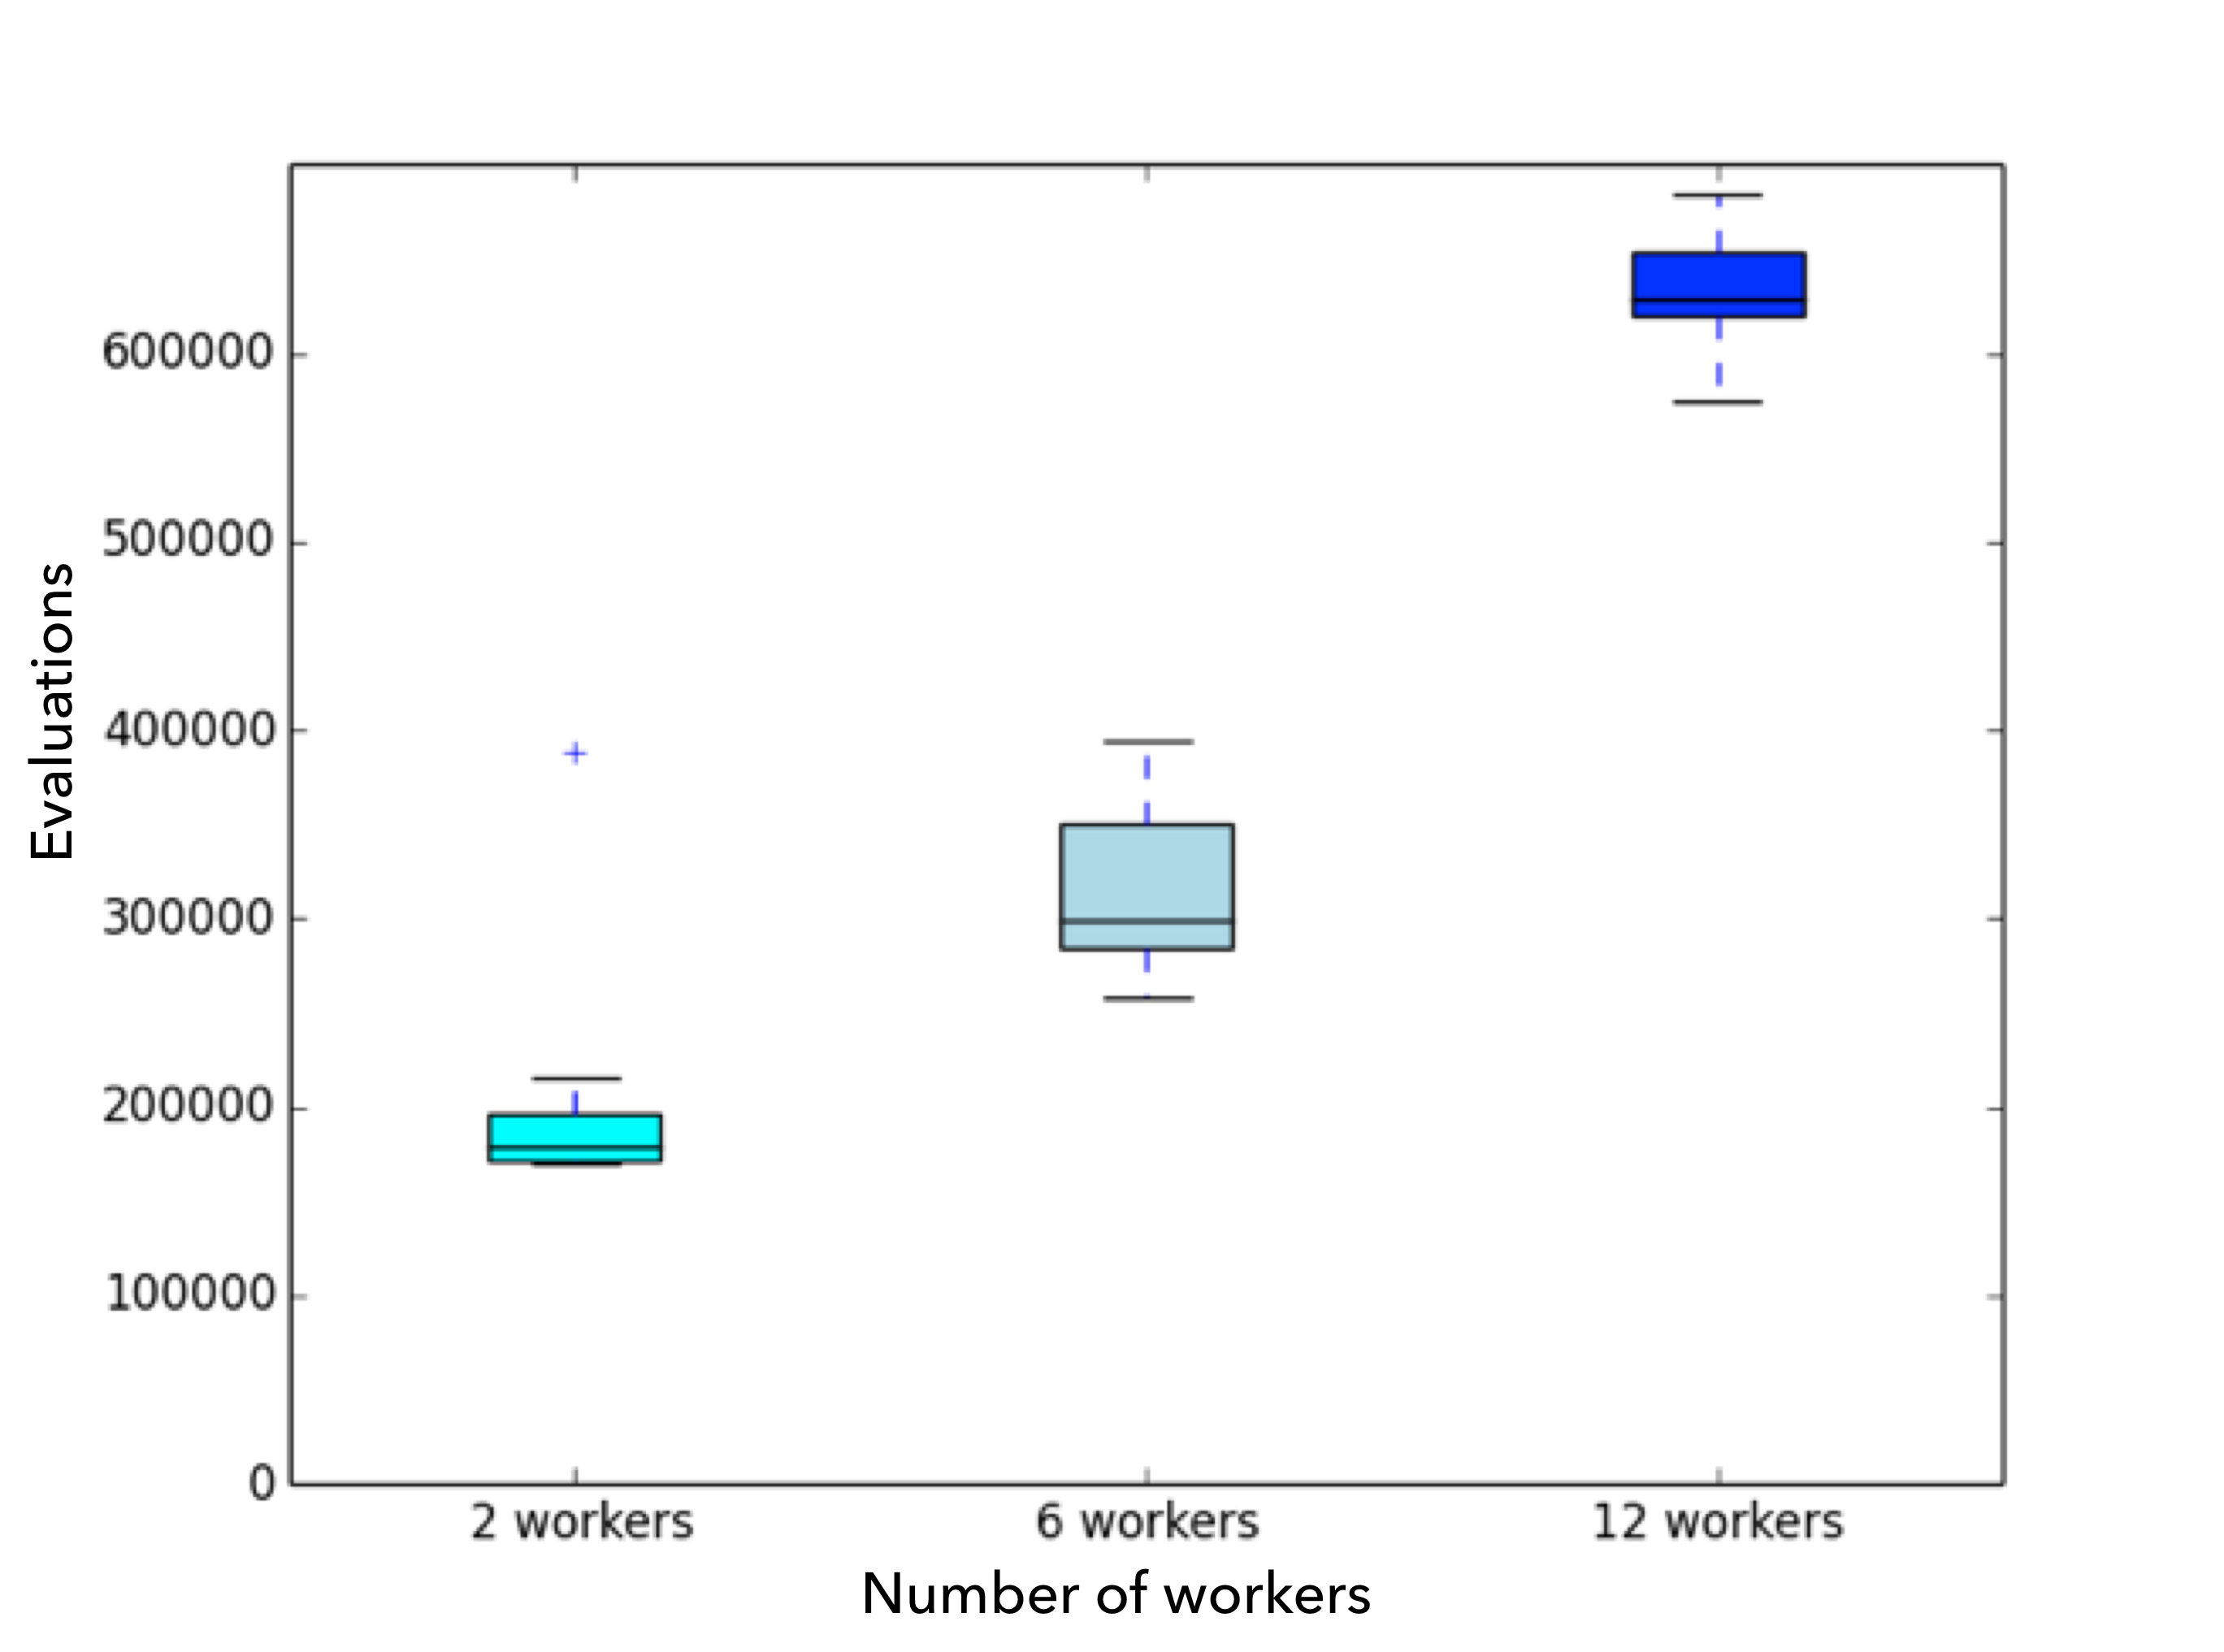
\includegraphics[width=3in]{img/schaffer_evals_homo.png}
    }
    \subfigure  [Heterogeneous]
    {
        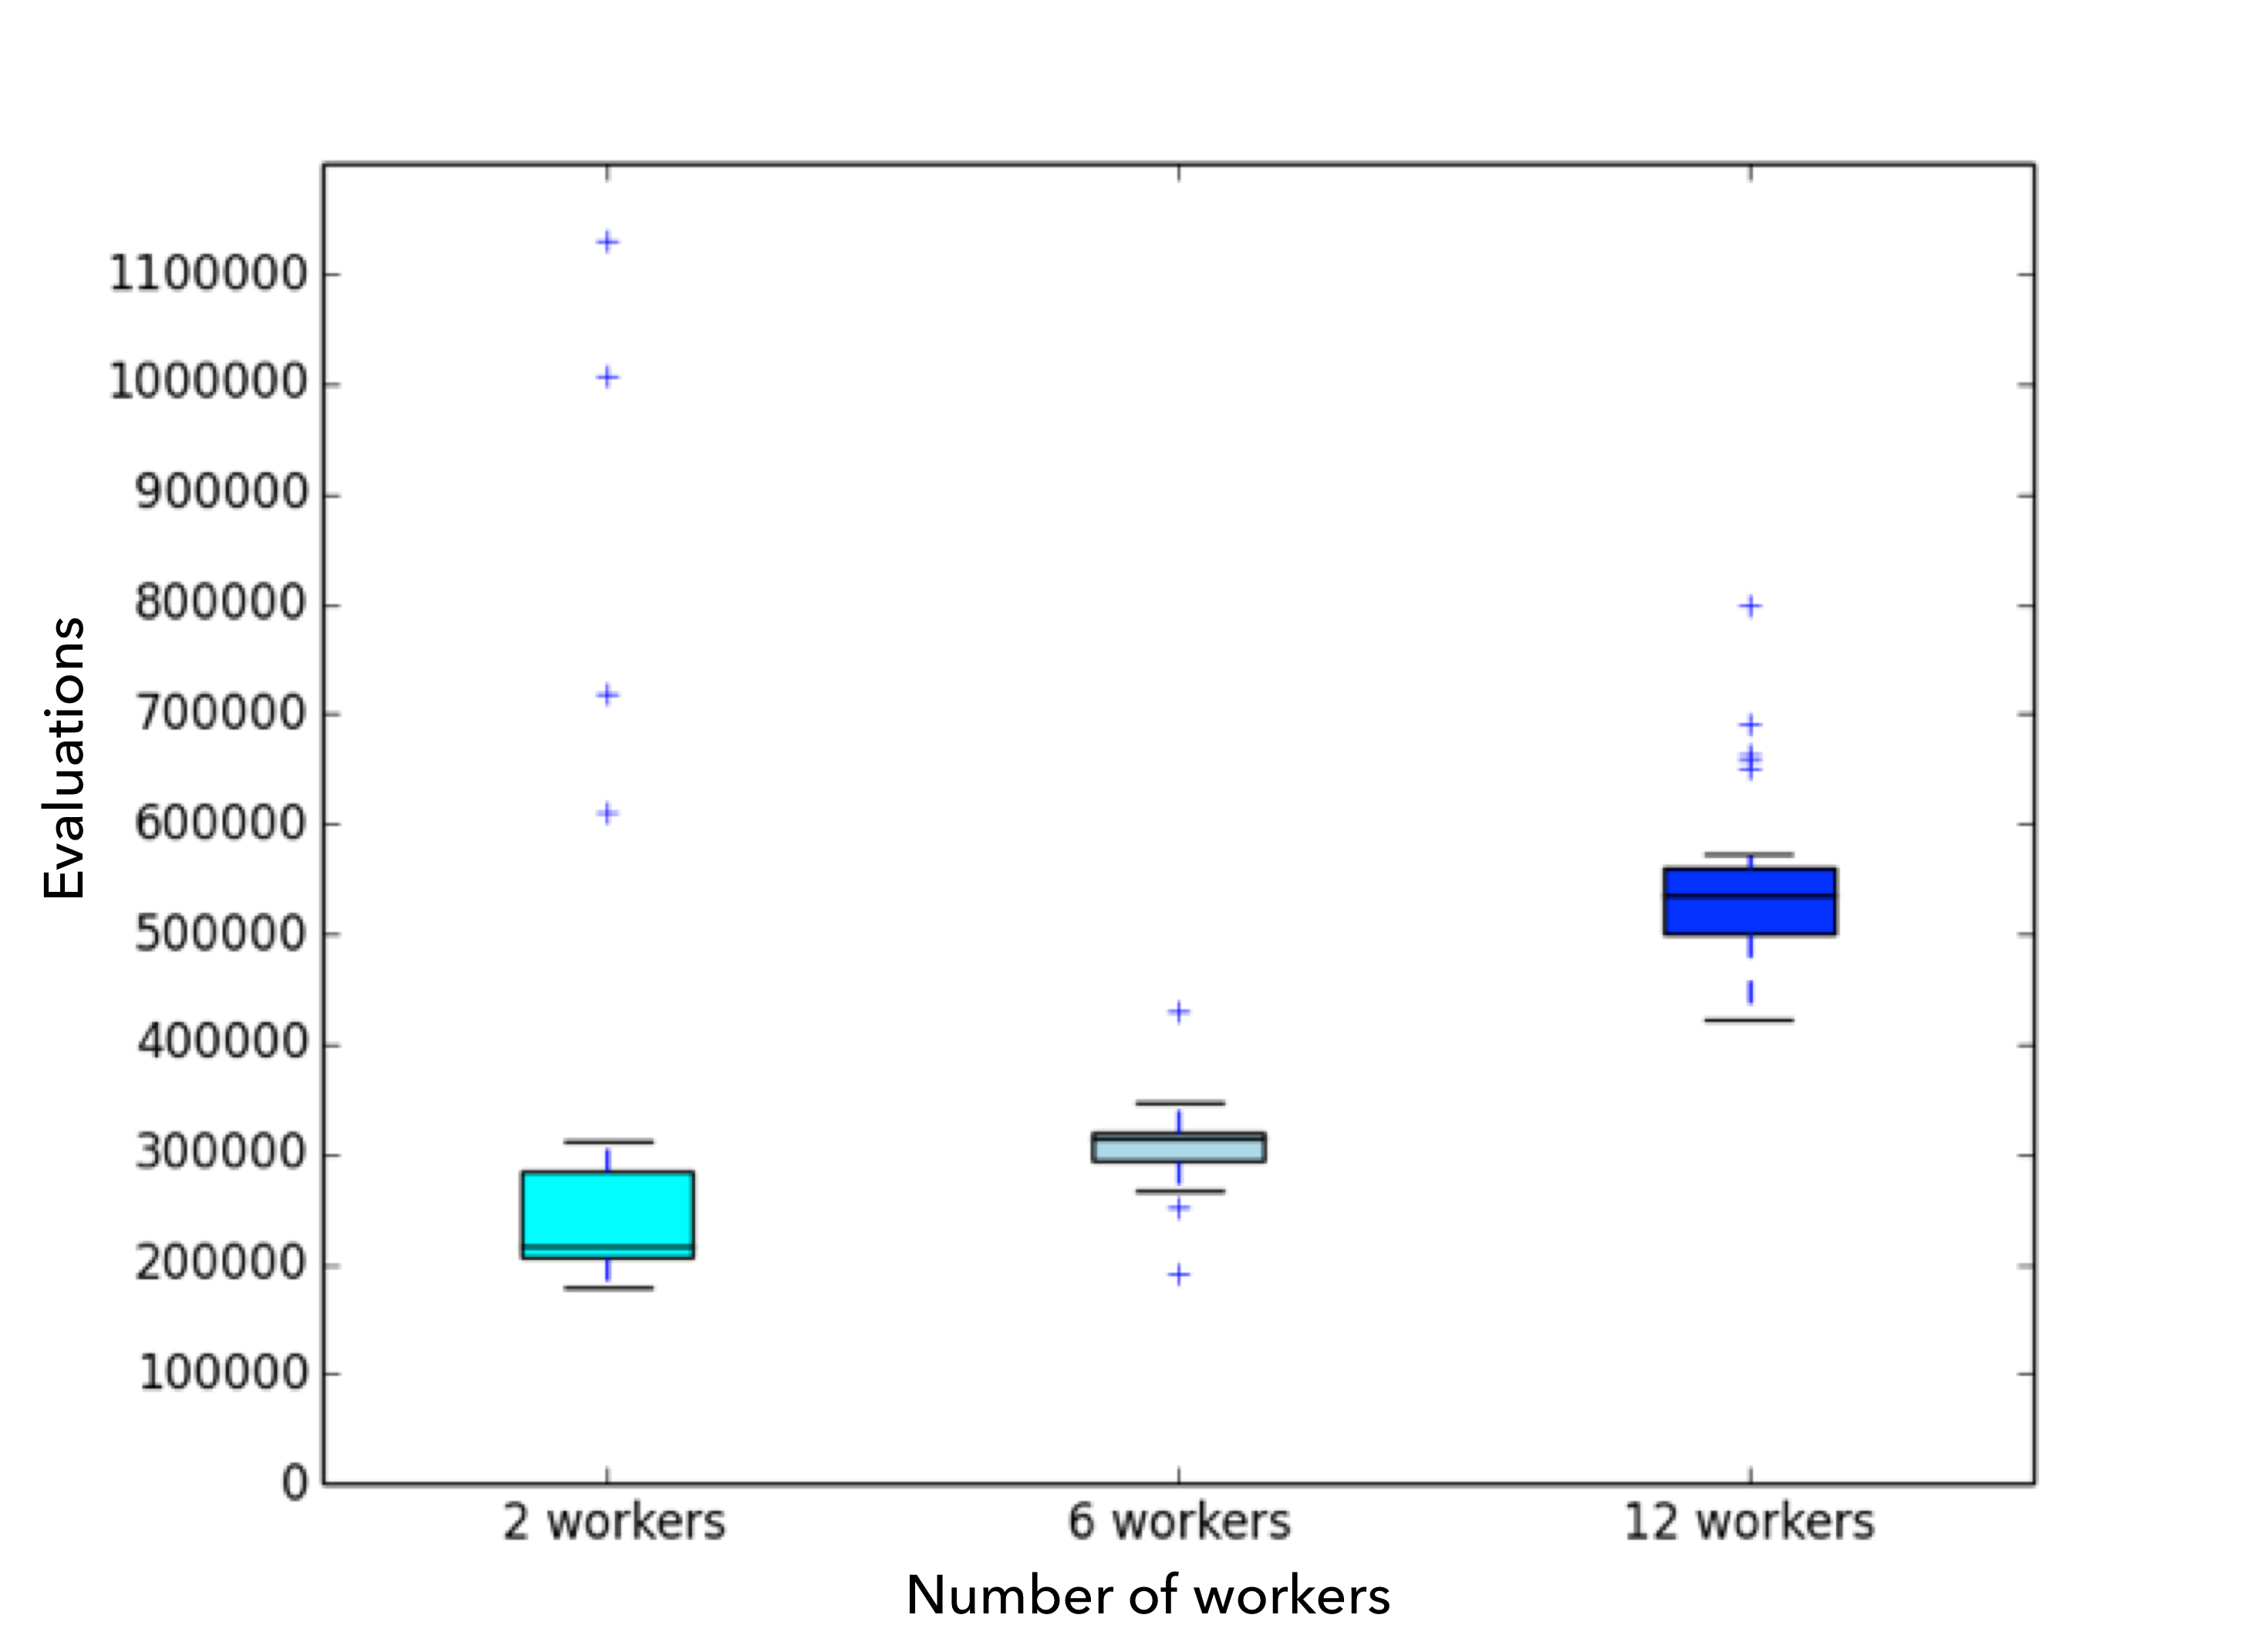
\includegraphics[width=3in]{img/schaffer_evals_hetereo.png}
    }


    \caption{Box-plot of the number
      of evaluations needed to reach a solution for the Schaffer function, with an (a)
      Homogeneous configuration, and (b) Heterogeneous
      configuration. Please note that $y$ scales are different.}
    \label{fig:schaffer}
\end{figure*}
%
\begin{table*}[t]
  \centering
  \caption{Summary of results obtained for the five floating point
      optimization problems. Best time per function is highlighted in bold.}
    \label{fig:summary}
    \begin{tabular}{|l|l|ccc|ccc|}
      \hline 
      \multirow{2}{*}{Function} & \multirow{2}{*}{Number of EvoWorkers} &  \multicolumn{3}{|c|}{Heterogeneous} & \multicolumn{3}{|c|}{Homogeneous}\\
      \cline{3-8}
                                & & 2 & 6 & 12 & 2 & 6 & 12\\
            \hline 
      \multirow{2}{*}{Ackley} & Mean time & 8.48&  5.707& {\bf 5.290} & 100.595 & 52.171 & 65.2023\\

                                & Mean evaluations & 27534.30 & 40239.66 & 60466.16 & 47645.9 & 81388.9 & 132308.6 \\
      \hline 
      \multirow{2}{*}{Rastrigin} & Mean time &  128.486207 & 36.847931 & 14.43517241 & 8.46793103 & 11.8510345 &  {\bf 4.43517241} \\

                                & Mean evaluations & 457148.552 & 347344.379 & 218830.552 & 31697.6897 & 105434.966 & 56090.7931 \\
      \hline
      \multirow{2}{*}{De Jong} & Mean time & 37.2465517 & 17.382069 & {\bf 17.6596552} & 33.1886207 & 19.77 & 27.2806897 \\


                                & Mean evaluations & 156795.276 & 213783.345 & 330531.828 & 159259.655 & 281918.034 & 651978.345 \\
      \hline
      \multirow{2}{*}{Griewank} & Mean time & 8.27241379 & 5.5337931 & {\bf 5.30482759} & 7.645667 & 5.716667 & 5.617333 \\


                                & Mean evaluations & 23688.8966 & 37118.1034 & 59249.2759 & 25779.6 & 42953.33 & 70536.53 \\
            \hline

      \multirow{2}{*}{Schaffer} & Mean time &  89.6493103 & 37.3044828 & {\bf 29.8093103} & 55.2410345 & 34.4448276 & 36.7113793 \\

                                & Mean evaluations & 316702.552  & 338147.103 & 545480.793 & 191024.759 & 311083.276 & 637198.31 \\
            \hline

       \end{tabular}

\end{table*}

The same steps as the previous section were followed when evaluating the five real valued
optimization problems of this section.  For brevity only two representative functions are
presented with figures, and summary of all the results are shown in
\autoref{fig:summary}. As we have done in \autoref{ss:onemax},
the first step is to tune the parameters for the homogeneous
configuration, which, once again, is done for the purposes of
establishing baseline values with which an heterogeneour configuration
can compare.
In \autoref{fig:griewank}, the results of the tuning phase for 6 and 12 workers
for the Griewank function are shown. For 12 workers results are not as flat as before,
with times comparable to the 6-worker configuration in the best case.

To compare the performance of the homogeneous approach and the heterogeneous approach based on RPW,
Figure \ref{fig:griewank-evals} compares the approaches with respect to the number of function evaluations required to find the optimal solution (within a 7 figure accuracy).
These results show a clear performance improvement, with the heterogeneous configuration
reducing the total number of function evaluations required to find a solution,
independently of the number of workers used.
On the other hand, for the Schaffer function, performance is quite similar,
with the heterogeneous approach only providing a slight reduction in the number
of function evaluations for the case with 12 EvoWorkers.
In the summary shown in Table ~\ref{fig:summary} two extreme cases are found, the Ackley and Rastrigin functions.
In the former, the heterogeneous configuration achieves the best performance, while the opposite is true on the latter.
Finally, performance on the De Jong function also favors the heterogeneous configurations.
Although the heterogeneous configuration performed poorly with the Rastrigin
function, especially when using two workers, the performance improved as we
added more workers.  The increased performance was on both the mean number of
evaluations and time to solution.


\section{Conclusions and Further Work}
\label{sec:conclusions}

The main objective of this paper was to prove the efficiency of
randomized pool-based evolutionary algorithms in a wide range of
benchmarks, from a simple OneMax Problem to more complicated, and
common, floating-point benchmarks, which are also evaluated in a wide
range of problem sizes, and results prove that this RPW approach is
able to find solutions in a competitive number of evaluations without
using significantly more resources than fixed-parameter workers,
something which is quite important in a cloud environment. By {\em
competitive} we mean that it is in the same ballpark as other tuned by
hand; however, our objective in this paper was to make the life of the
researcher easier by reducing the number of parameters that need to be
tuned. Since experimental design is measured on researcher's, not
computer's time, it is much more valuable and, anyways, the
experiments needed to find the best parameters take, themselves,
computer time which, in a cloud environment, is also worth money. So,
even if performance of this RPW algorithm is almost always better than
that in a fine-tuned, homogeneous, algorithm, this saves the need of
computationally expensive meta-algorithms, while at the same time
allowing to keep a high diversity level in throughout all
subpopulations.  Results also show that the benefits of a random
parametrization strategy are not only present when using an
heterogeneous approach, even a random homogeneous configuration could
bring benefits.

Unfortunately the RPW strategy is not a silver bullet, as there are cases
when it might not find the solution using the minimum number of
evaluations; and even when it does, it needs marginally more time to
reach it. However these disadvantages are
offset by the fact that it comes very close to zero parameter tuning,
giving a consistently good result across a good range of problem
instances. Tuning is still needed for population-level parameters such
as population size, the RPW-specific sample-size, as well as other
parameters related to them; however, parameters for evolutionary
operators have been totally eliminated, making it easier to use for
non-experienced researchers or as part of evolutionary algorithm
frameworks.

The worst result is achieved for the Rastrigin function, which
is one of the most difficult ones; not only the time needed is worse,
also the number of evaluations. In case such as these it would be
interesting to use some technique to constrain the range of variation
of the random parameters or to investigate additional operators that
would work better across a wide range of situations.

The work presented in this paper, thus, gives further proof to our
previous evaluation of randomly parametrized workers, inspired
initially by the work of Fukunaga et al. \cite{fuku1}; it also shows that the random
parametrization is a technique that, by itself, is efficient in
multi-population nature-inspired algorithms, independently of the type
of algorithm or how population or work is distributed. In general, we
can conclude that 
random parametrization will allow a good initial result for most
problems, providing a fast solution in cases where there is not enough
time to perform optimization of the parameters in a parallel
setup. Besides, it also lowers the amount of ``islands'' (in our case
workers) needed for a randomized parameter setting strategy to work:
while in the case of Fukunaga et al. \cite{fuku1} a large number of islands was
needed, in our case just a few of them, or even only two, are
enough.

This work also opens new avenues of research in the future. We are
randomizing every worker separately, but every one has a static
parametrization. In principle, it would be possible also to change
this parametrization after several generations, which might have a
positive effect in diversity and search space exploration. The range
of variation of the parameters is static, but it could also be varied
adaptively, so that as evolution progresses, exploitation is used more
heavily than exploration. Increasing the amount of EvoWorkers might
have an interesting effect from the point of view of efficiency in
difficult problems such as the Schaffer function, so that will be
another possible line of future work.
Finally, other operators such as
BLX-$\alpha$ could be added to the mix, which might have a good effect
on performance.


\section*{Acknowledgements}

This paper has been supported in part by projects DeepBio (TIN2017-85727-C4-2-P)
and TecNM-5654.19-P.
% This should be updated


%----------------------------------------------------------------------------------------
%	REFERENCE LIST
%----------------------------------------------------------------------------------------
\bibliographystyle{IEEEtran}
\bibliography{biblio,evospace-i,parameters,volunteer,geneura}


%----------------------------------------------------------------------------------------

\end{document}
